\documentclass[a4paper,12pt]{article}

%Class
	%\documentclass[a4paper,12pt]{article}

%Packages
	\usepackage{amsmath}					% Standard maths
	\usepackage{amssymb}					% Standard maths
	\usepackage{amsthm}						% Standard maths
	\usepackage{thmtools, thm-restate}% Theorem styles
	\usepackage{mathtools}
	\usepackage[newzealand]{babel}% Date/time in British format (yes, I know it says NZ)
	\usepackage{datetime}					% Date/time
	\usepackage{multirow}					% For stacked subscripts
	\usepackage{xcolor}						% For colour!
	\usepackage[normalem]{ulem}		% For strikeout
	\usepackage{isomath}
	\usepackage{fancyhdr}					% For the headers
	\usepackage{mfirstuc}					% For the headers
	\usepackage[hmargin=1in,top=0.8in,bottom=1in]{geometry} % Page margins more reasonable
	\usepackage{graphicx}					% For including graphics
	%\usepackage{float}						% For something
	\usepackage{enumitem}					% For numbering tweaks
	\usepackage{pgfplots}
	\usepackage[margin=15pt,font={footnotesize},labelfont=bf,format=hang]{caption}
\usepackage[margin=15pt,font={footnotesize},labelfont=bf,format=hang]{subcaption}
	\usepackage{url}
	\usepackage[hidelinks]{hyperref}	% For hyperlinks
	\usepackage{breakurl}
	\usepackage{cleveref}
	\usepackage[scaled=.92]{helvet}
	\newbool{show_question}
	\newbool{show_solution}
	\newcommand{\solutioninheading}{\ifbool{show_solution}{: SOLUTIONS}{}}
	\usepackage{pgfplots}
\newcommand{\ep}{\varepsilon}

\makeatletter 
\newcommand\mynobreakpar{\par\nobreak\@afterheading} 
\makeatother

    \newcommand{\question}[3]{
    	\item \textbf{#1} \mynobreakpar \nobreak \medskip % Title
    	%
    	\ifbool{show_question}{\nobreak#2}{} % Question
    	%
    	%
    	\ifbool{show_question}{\ifbool{show_solution}{\par\medskip\textbf{Solution:}}{}}{} % Both
    	\ifbool{show_solution}{#3}{} % Answer
    }			

%MATHEMATICAL SHORTCUTS
%Two and three-part definitions
	\newcommand{\twopartdef}[4]
	{	\left\{
			\begin{array}{ll}
				#1 & \mbox{if } #2 \\
				#3 & \mbox{if } #4
			\end{array}
		\right.}
%	\newcommand{\threepartdef}[6]
%	{	\left\{
%			\begin{array}{ll}
%				#1 & \mbox{if } #2 \\
%				#3 & \mbox{if } #4 \\
%				#5 & \mbox{if } #6
%			\end{array}
%		\right.}
%Blackboard bold	
	\newcommand{\N}{{\mathbb N}} 
	\newcommand{\R}{{\mathbb R}} 
	\newcommand{\C}{{\mathbb C}} 
	%Curly letters
%	\newcommand{\E}{{\mathcal E}}	
%	\newcommand{\F}{{\mathcal F}} 
%	\newcommand{\Null}{{\mathcal N}} 
%	\newcommand{\R}{\mathcal{R}} 
%	\newcommand{\Z}{\mathcal{Z}} 
%Uprights
	\newcommand{\D}{{\mathrm D}}
	\renewcommand{\d}{{\mathrm d}}
%Easy Greeks
%	\def\a{\alpha}
%	\def\g{\gamma}
%	\newcommand{\e}{{\varepsilon}}
%	\newcommand{\la}{{\lambda}}  
%	\newcommand{\om}{{\Omega}}
	\renewcommand{\epsilon}{\varepsilon}
	
%Vector operators
	\def \p {\partial}
	\newcommand{\del}{{\nabla}}
	\newcommand{\grad}{{\nabla}}
    \newcommand{\vdel}{\boldsymbol{\nabla}}
    \newcommand{\vgrad}{\boldsymbol{\nabla}}
    \newcommand{\vnabla}{\boldsymbol{\nabla}}
	\newcommand{\cross}{{\times}}
	\newcommand{\Lap}{{\nabla^2}} 
%Arrows
%	\newcommand{\goesto}[1]{\xrightarrow[#1]{}}
%hats
%	\newcommand{\nhat}{\widehat{\v{n}}}
%	\newcommand{\shat}{\widehat{\v{s}}}
	\renewcommand{\hat}{\widehat}
%Note to self
%	\newcommand{\note}[1]{[\textbf{\textsl{\MakeUppercase{#1}}}]}
	
%Stress tensor
%	\newcommand{\T}{\vg{\sigma}}

% Vectors, quaternions etc.
\renewcommand{\v}[1]{\mathbfit{#1}}      % Generic vector
\newcommand{\vc}[1]{\bm{\mathcal{#1}}}      % vector mathcal
\newcommand{\uv}[1]{\widehat{\mathbfit{#1}}}      % Generic unit vector
\newcommand{\q}[1]{\mathsfbfit{#1}}        % Generic quaternion
\renewcommand{\t}[1]{\mathsfbfit{#1}}	 % Generic tensor
\newcommand{\m}[1]{\mathsfbfit{#1}}	 % Generic matrix
\newcommand{\vu}[1]{\mathbf{#1}}         % Upright vector (for zero vector)
\newcommand{\qu}[1]{\mathbf{#1}}       % Upright quaternion (for zero quaternion)
\newcommand{\tu}[1]{\bm{\mathsf{#1}}}	 % Upright tensor (for zero tensor)

%Real and imaginary
\renewcommand{\Re}{\operatorname{Re}}
\renewcommand{\Im}{\operatorname{Im}}
	
%Non-dim numbers
%	\renewcommand{\Re}{\operatorname{Re}}
%	\newcommand{\Bi}{\operatorname{Bi}}
%	\newcommand{\Fo}{\operatorname{Fo}}
	
%Misc
\DeclareMathSymbol{\Delta}{\mathalpha}{operators}{1} % Keeps Delta upright
\DeclareMathSymbol{\Gamma}{\mathalpha}{operators}{0} % Keeps Gamma upright
	\newcommand{\cosec}{\operatorname{cosec}}
	\newcommand{\cosech}{\operatorname{cosech}}
	\newcommand{\sech}{\operatorname{sech}}
	\newcommand{\tr}{\operatorname{tr}}
	\newcommand{\erf}{\operatorname{erf}}
	\newcommand{\order}{\mathcal{O}}
%	\newcommand{\V}{\mathcal{V}} % 	CurlyV = (Bi V) / (1 + Bi)

% Differentiating 
\newcommand{\fd}[2]{\mathchoice{\frac{\d #1}{\d #2}}{\d #1/\d #2}{\d #1/\d #2}{\d #1/\d #2}}
\newcommand{\fdd}[2]{\mathchoice{\frac{\d^2 #1}{\d #2^2}}{\d^2 #1/\d #2^2}{\d^2 #1/\d #2^2}{\d^2 #1/\d #2^2}}
\newcommand{\fddd}[2]{\mathchoice{\frac{\d^3 #1}{\d #2^3}}{\d^3 #1/\d #2^3}{\d^3 #1/\d #2^3}{\d^3 #1/\d #2^3}}
\newcommand{\fdddd}[2]{\mathchoice{\frac{\d^4 #1}{\d #2^4}}{\d^4 #1/\d #2^4}{\d^4 #1/\d #2^4}{\d^4 #1/\d #2^4}}
\newcommand{\fdn}[3]{\mathchoice{\frac{\d^{#1} #2}{\d #3^{#1}}}{\d^{#1} #2/\d #3^{#1}}{\d^{#1} #2/\d #3^{#1}}{\d^{#1} #2/\d #3^{#1}}}
\newcommand{\pd}[2]{\mathchoice{\frac{\p #1}{\p #2}}{\p #1/\p #2}{\p #1/\p #2}{\p #1/\p #2}}
\newcommand{\pdd}[2]{\mathchoice{\frac{\p^2 #1}{\p #2^2}}{\p^2 #1/\p #2^2}{\p^2 #1/\p #2^2}{\p^2 #1/\p #2^2}}
\newcommand{\pddmixed}[3]{\frac{\p^2 #1}{\p #2 \p #3}}
\newcommand{\pddd}[2]{\frac{\p^3 #1}{\p #2^3}}
\newcommand{\pdn}[3]{\mathchoice{\frac{\p^{#1} #2}{\p #3^{#1}}}{\p^{#1} #2/\p #3^{#1}}{\p^{#1} #2/\p #3^{#1}}{\p^{#1} #2/\p #3^{#1}}}
	
	% Misc
\newcommand{\e}{\mathrm{e}}
\renewcommand{\i}{\mathrm{i}}
\newcommand{\dx}{\,\mathrm{d}x}
\newcommand{\dy}{\,\mathrm{d}y}
\renewcommand{\epsilon}{\varepsilon}
\renewcommand{\Re}{\operatorname{Re}}
\newcommand{\Four}{\mathcal{F}}

\newcommand{\mat}[4]{\begin{pmatrix}#1 & #2 \\ #3 & #4 \end{pmatrix}}

	%Column vectors
	\makeatletter
\newcommand\rcvector[2][\\]{\ensuremath{%
  \global\def\rc@delim{#1}%
    \negthinspace\begin{pmatrix}
      \rc@vector #2,\relax\noexpand\@eolst%
    \end{pmatrix}}}
\def\rc@vector #1,#2\@eolst{%
  \ifx\relax#2\relax
    #1
  \else
    #1\rc@delim
    \rc@vector #2\@eolst%
  \fi}
\makeatother

\newcommand{\colvec}{\rcvector}
\newcommand{\rowvec}{\rcvector}
\renewcommand{\binom}{\rcvector}
	
	%Colours
%	\newcommand{\orange}[1]{{\color{orange} #1 }}
%	\newcommand{\blue}[1]{{\color{blue} #1 }}

%Theorem styles
%	\declaretheoremstyle[headpunct={\:\:\:}, shaded={bgcolor={rgb}{0.9,0.9,0.9}, margin=5pt}]{problem}
%	\declaretheoremstyle[headpunct={\:\:\:}, shaded={rulecolor=black, rulewidth=0.4pt, bgcolor={rgb}{1,1,1}, margin=5pt}]{definition}
%	\declaretheoremstyle[headpunct={\:\:\:}, spaceabove=15pt, notefont=\bf, notebraces={(}{)}]{theorem}
%	\declaretheoremstyle[headpunct={\:\:\:}, numbered=no, spaceabove=15pt, qed={\checkmark}]{solution}
%	
%	\declaretheorem[style=definition,numberwithin=section]{definition}
%	\declaretheorem[numberlike=definition, style=theorem]{theorem}
%	\declaretheorem[numberlike=definition, style=theorem]{lemma}
%	\declaretheorem[numberlike=definition,style=problem]{problem}
%	\declaretheorem[numberlike=definition, style=theorem]{proposition}
%	\declaretheorem[numberlike=definition, style=theorem]{corollary}
%	\declaretheorem[numberlike=definition, style=theorem]{remark}
%	\declaretheorem[numberlike=definition, style=theorem]{example}
%	\declaretheorem[numberlike=definition, style=theorem]{notation}
%	\declaretheorem[style=solution]{solution}

%Depth of display breaks to allow	
	\allowdisplaybreaks[1]

%How deep do we want the Table of Contents to go?	
%	\setcounter{tocdepth}{1}

%Sections
\makeatletter
\renewcommand{\section}{\@startsection
{section}%                   % the name
{1}%                         % the level
{0mm}%                       % the indent
{-\baselineskip}%            % the before skip
{0.5\baselineskip}%          % the after skip
{\normalfont\bfseries}} % the style
\makeatother

% Wavy underline
\makeatletter
\font\sixly=lasyb10 scaled 1200
\def\tinners{\bgroup \markoverwith{\lower8.5\p@\hbox{\sixly \char58}}\ULon}
\makeatother
\newcommand{\answer}[1]{\tinners{\; #1 \;}}

%Setting the footnotes to use *,**,+ etc rather than 1,2,3	
\renewcommand{\thefootnote}{\fnsymbol{footnote}}

%Italic quote environment
%\newenvironment{quoteitalic}{\begin{quote}\itshape}{\end{quote}}

%Heading
\newcommand{\heading}[2]{
\setlength{\parindent}{0pt}
\textbf{MATH3171 (Mathematical Biology III)}

\textbf{YEAR 2025--26, \MakeUppercase{#1} TERM}
\setlength{\parskip}{3ex}

\textbf{\MakeUppercase{#2}}
%
\setlength{\parskip}{2ex}

}

%========================================================================================================================
%DOCUMENT BEGINS HERE!

\usepackage{multicol}
\setbool{show_question}{true}
\setbool{show_solution}{true}
\begin{document}
%
\heading{Michaelmas}{Problems class 2\solutioninheading}

\ifbool{show_solution}{}{
  In this problems class we are going to practise drawing and interpreting graphs: phase portraits for two-dimensional systems and bifurcation diagrams. Phase portraits allow us to see the long-term behaviour of our systems for all possible initial conditions; whereas bifurcation diagrams tell us about the existence/stability of equilibria for different parameter values.
}

\begin{enumerate}[label={\bf \arabic{*}.\;}, ref={\arabic{*}},itemsep=3ex, left=0ex]

    % Q1
    \question{Phase portrait recipe}
    { % Question
      Linear stability analysis is an algebraic method to determine the stability of a system's equilibria. Phase portraits are a graphical method which can often also imply the same stability. Think of them as complementary tools. A recipe for drawing a phase portrait is:
      \begin{enumerate}[label=(\roman*)]
        \item Compute and draw equilibria, indicating stability from a linear stability analysis if you have done one.
        \item Draw nullclines ($\dot{x} = 0$, $\dot{y} = 0$):
          \begin{itemize}
            \item Trajectories along $\dot{x}=0$ will be vertical,
            \item Trajectories along $\dot{y}=0$ will be horizontal.
          \end{itemize}
          Equilibria will be where $\dot{x}=0$ and $\dot{y}=0$ nullclines intersect.
        \item Test the regions between the nullclines for $\dot{x}, \dot{y} \gtrless 0$.
        \item Infer direction of trajectories and join up.
      \end{enumerate}

      Trajectories in a phase portrait do not intersect: can you explain why?
    }
    { % Solution
      Trajectories in a phase portrait do not intersect, because where they intersect, the trajectory (i.e.\ value of $(\dot{x},\dot{y})$) should be unique in a deterministic (i.e.\ non-random) system.
    }

    % Q2
    \question{Trajectory drawing practice}
    { % Question
      Consider the half-completed phase portrait below for the system $(x,y)$. Identify the equilibria and complete the testing of the regions. Then draw in the trajectories and infer the stability of the equilibria.
      \begin{center}
        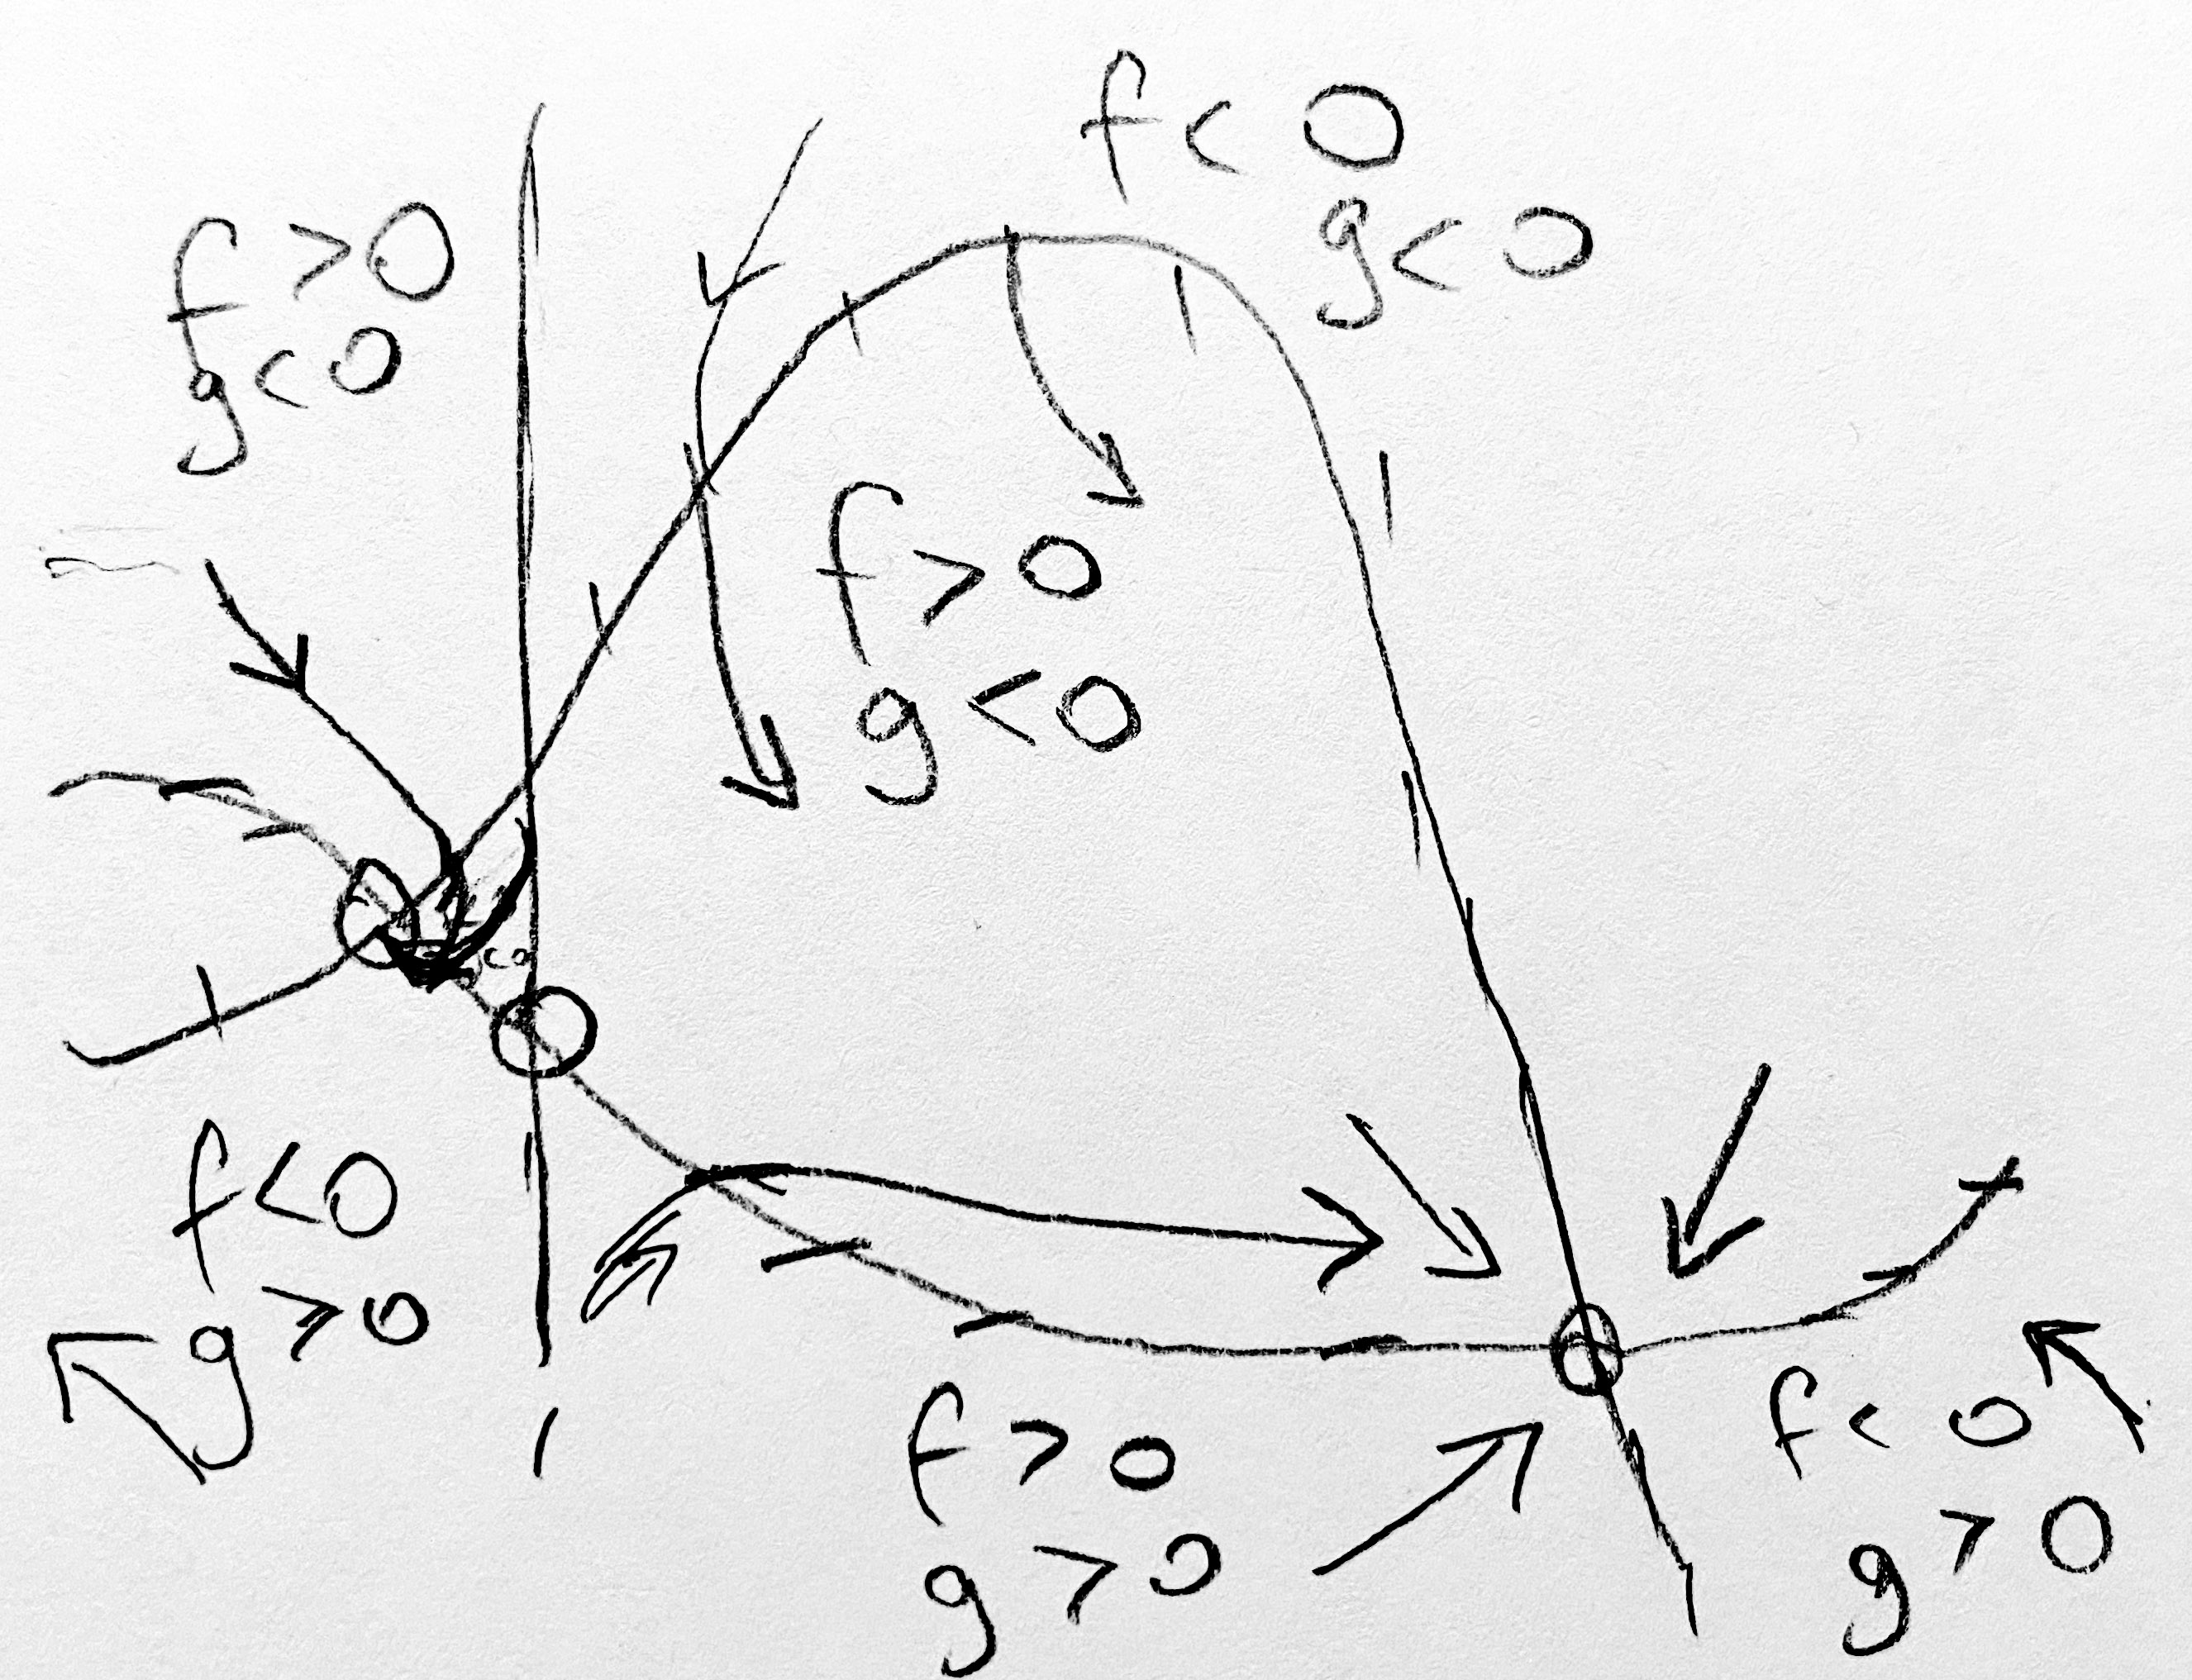
\includegraphics[scale=1.2]{images/nullclines-exercise}
      \end{center}
    }
    { % Solution
      \begin{center}
        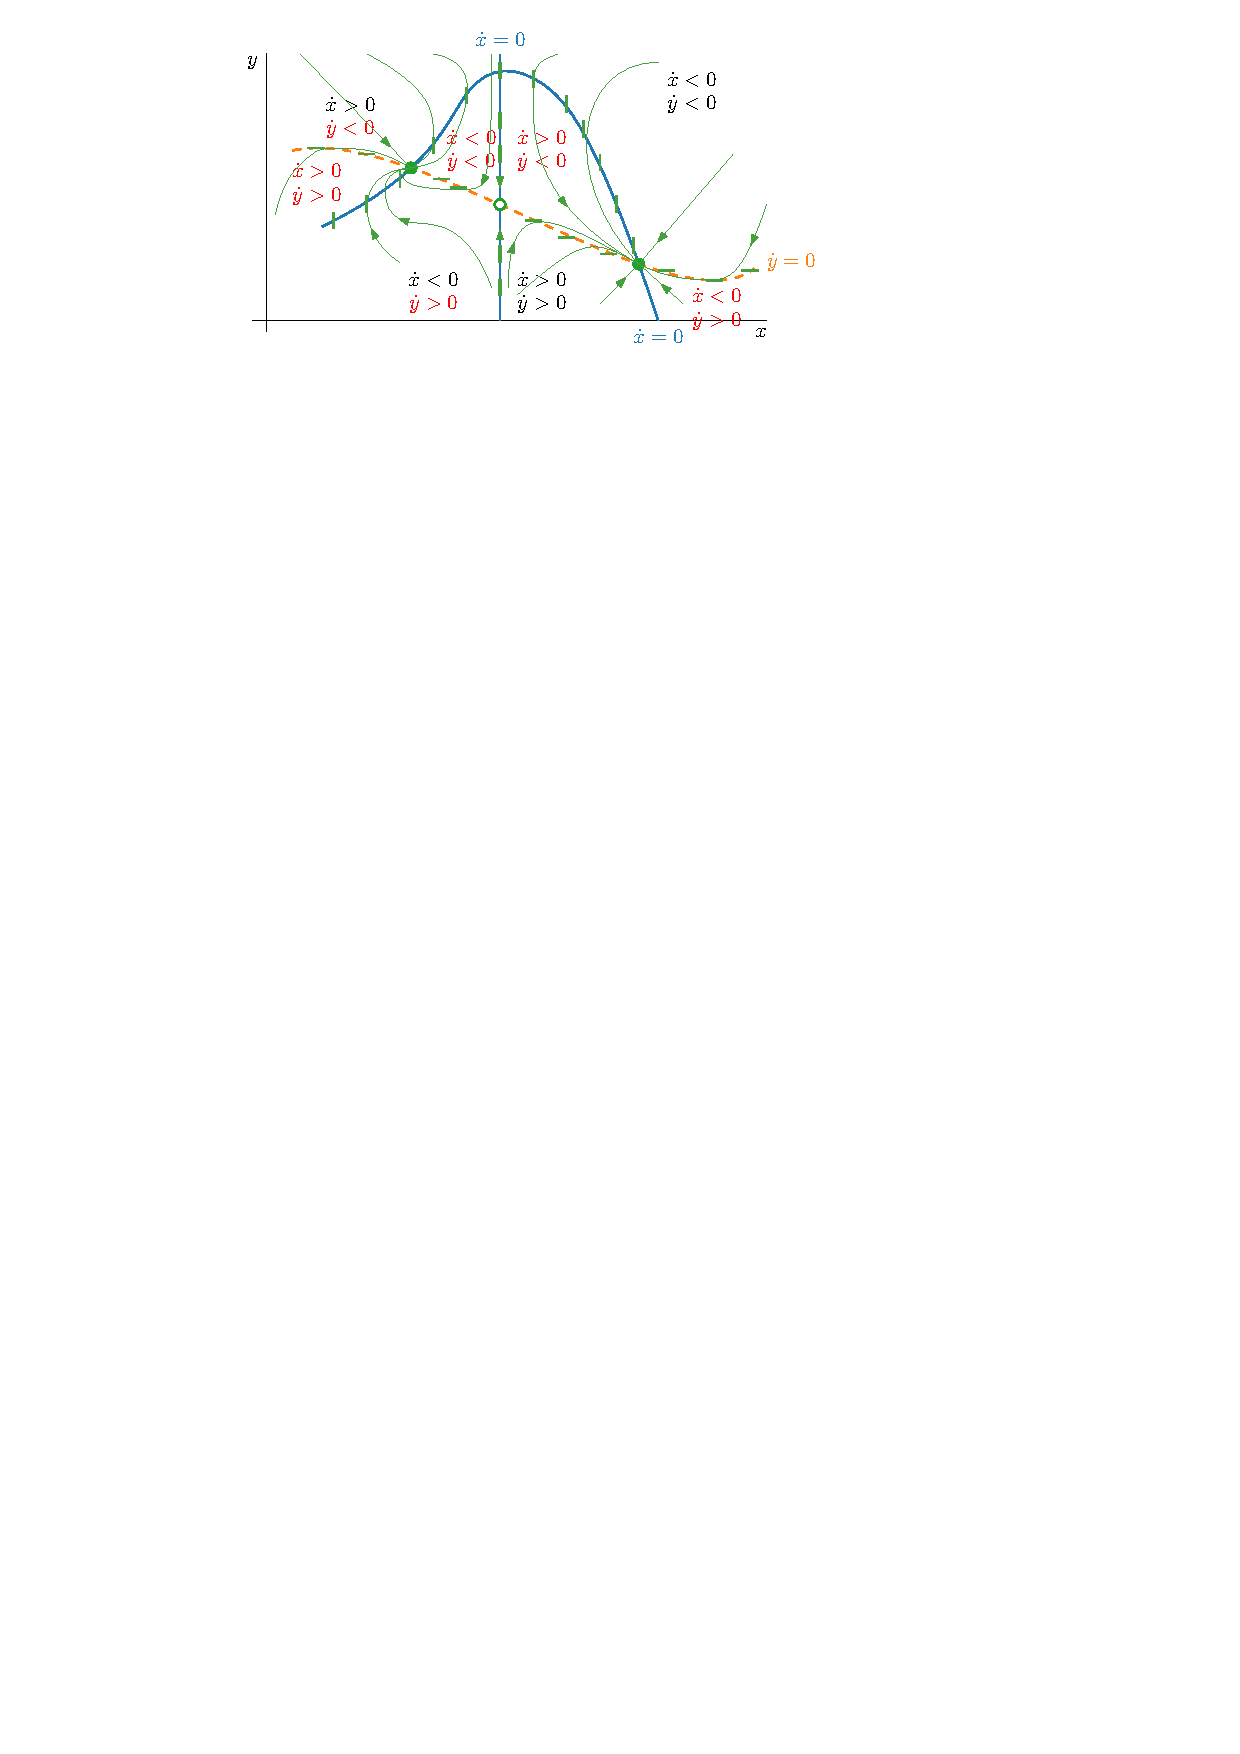
\includegraphics[width=13cm]{images/nullclines-exercise-sol2.pdf}
      \end{center}
    }
    %\newpage
    %Q3
    \question{Bifurcation investigation (Exam 2023)}
    {
    \begin{multicols}{2}
    	Consider the bifurcation diagram on the right, which shows how the equilibria $x_0$ of a single-species population model depend on a single parameter, $k$:

    \begin{enumerate}
        \item Write down all the equilibria, $x_0$, shown on the graph.
	    \item Hence write down a model for a population $x(t)$ in the form
	\[ \fd{x}{t}=f(x,k) \]
	which would produce this bifurcation diagram. 
    \end{enumerate}
    
    	\begin{center}
        \vspace{3mm}
		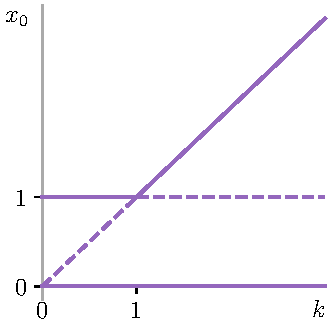
\includegraphics{images/bifurcation.pdf}
	\end{center}
    
    \end{multicols}
	}
	{
	    For each value of $k$, there are three values of $x_0$:
    \begin{equation*}  
        x_0 = 0, \quad k, \quad \text{and } 1.
    \end{equation*}
    This suggests an equation of the form
    \begin{equation*}
        \fd{x}{t} = -x(x-k)(x-1),
    \end{equation*}
    i.e.\ the Allee model seen in class. 
    Drawing the portrait confirms the stability.

	}


    % Q4
    \question{Competitive Lotka--Volterra}
    { % Question
      Recall from last week's lectures that the competitive Lotka--Volterra system, in nondimensional form, looks like
      \begin{align}
        \fd{x}{t} &= x(1-x-\gamma_1 y),\\
        \fd{y}{t} &= \beta y (1-y-\gamma_2 x),
      \end{align}
      with $\beta,\gamma_1, \gamma_2 > 0$.

      Drawing on the nullclines and equilibria for the $\gamma_1>1$, $\gamma_2>1$ gives us
      %
      \begin{center}
        %% Creator: Matplotlib, PGF backend
%%
%% To include the figure in your LaTeX document, write
%%   \input{<filename>.pgf}
%%
%% Make sure the required packages are loaded in your preamble
%%   \usepackage{pgf}
%%
%% and, on pdftex
%%   \usepackage[utf8]{inputenc}\DeclareUnicodeCharacter{2212}{-}
%%
%% or, on luatex and xetex
%%   \usepackage{unicode-math}
%%
%% Figures using additional raster images can only be included by \input if
%% they are in the same directory as the main LaTeX file. For loading figures
%% from other directories you can use the `import` package
%%   \usepackage{import}
%%
%% and then include the figures with
%%   \import{<path to file>}{<filename>.pgf}
%%
%% Matplotlib used the following preamble
%%   \usepackage{fontspec}
%%   \setmainfont{DejaVuSerif.ttf}[Path=/Users/adam/opt/anaconda3/lib/python3.8/site-packages/matplotlib/mpl-data/fonts/ttf/]
%%   \setsansfont{DejaVuSans.ttf}[Path=/Users/adam/opt/anaconda3/lib/python3.8/site-packages/matplotlib/mpl-data/fonts/ttf/]
%%   \setmonofont{DejaVuSansMono.ttf}[Path=/Users/adam/opt/anaconda3/lib/python3.8/site-packages/matplotlib/mpl-data/fonts/ttf/]
%%
\begingroup%
\makeatletter%
\begin{pgfpicture}%
\pgfpathrectangle{\pgfpointorigin}{\pgfqpoint{3.000000in}{2.200000in}}%
\pgfusepath{use as bounding box, clip}%
\begin{pgfscope}%
\pgfsetbuttcap%
\pgfsetmiterjoin%
\definecolor{currentfill}{rgb}{1.000000,1.000000,1.000000}%
\pgfsetfillcolor{currentfill}%
\pgfsetlinewidth{0.000000pt}%
\definecolor{currentstroke}{rgb}{1.000000,1.000000,1.000000}%
\pgfsetstrokecolor{currentstroke}%
\pgfsetdash{}{0pt}%
\pgfpathmoveto{\pgfqpoint{0.000000in}{0.000000in}}%
\pgfpathlineto{\pgfqpoint{3.000000in}{0.000000in}}%
\pgfpathlineto{\pgfqpoint{3.000000in}{2.200000in}}%
\pgfpathlineto{\pgfqpoint{0.000000in}{2.200000in}}%
\pgfpathclose%
\pgfusepath{fill}%
\end{pgfscope}%
\begin{pgfscope}%
\pgfsetbuttcap%
\pgfsetmiterjoin%
\definecolor{currentfill}{rgb}{1.000000,1.000000,1.000000}%
\pgfsetfillcolor{currentfill}%
\pgfsetlinewidth{0.000000pt}%
\definecolor{currentstroke}{rgb}{0.000000,0.000000,0.000000}%
\pgfsetstrokecolor{currentstroke}%
\pgfsetstrokeopacity{0.000000}%
\pgfsetdash{}{0pt}%
\pgfpathmoveto{\pgfqpoint{0.436279in}{0.296600in}}%
\pgfpathlineto{\pgfqpoint{2.966667in}{0.296600in}}%
\pgfpathlineto{\pgfqpoint{2.966667in}{1.968025in}}%
\pgfpathlineto{\pgfqpoint{0.436279in}{1.968025in}}%
\pgfpathclose%
\pgfusepath{fill}%
\end{pgfscope}%
\begin{pgfscope}%
\pgfpathrectangle{\pgfqpoint{0.436279in}{0.296600in}}{\pgfqpoint{2.530388in}{1.671426in}}%
\pgfusepath{clip}%
\pgfsetbuttcap%
\pgfsetroundjoin%
\pgfsetlinewidth{0.702625pt}%
\definecolor{currentstroke}{rgb}{0.121569,0.466667,0.705882}%
\pgfsetstrokecolor{currentstroke}%
\pgfsetdash{{2.590000pt}{1.120000pt}}{0.000000pt}%
\pgfpathmoveto{\pgfqpoint{2.017771in}{0.296600in}}%
\pgfpathlineto{\pgfqpoint{0.436279in}{1.042772in}}%
\pgfusepath{stroke}%
\end{pgfscope}%
\begin{pgfscope}%
\pgfpathrectangle{\pgfqpoint{0.436279in}{0.296600in}}{\pgfqpoint{2.530388in}{1.671426in}}%
\pgfusepath{clip}%
\pgfsetbuttcap%
\pgfsetroundjoin%
\pgfsetlinewidth{0.702625pt}%
\definecolor{currentstroke}{rgb}{1.000000,0.498039,0.054902}%
\pgfsetstrokecolor{currentstroke}%
\pgfsetdash{{2.590000pt}{1.120000pt}}{0.000000pt}%
\pgfpathmoveto{\pgfqpoint{0.436279in}{1.341241in}}%
\pgfpathlineto{\pgfqpoint{1.565916in}{0.296600in}}%
\pgfusepath{stroke}%
\end{pgfscope}%
\begin{pgfscope}%
\pgfsetbuttcap%
\pgfsetroundjoin%
\definecolor{currentfill}{rgb}{0.000000,0.000000,0.000000}%
\pgfsetfillcolor{currentfill}%
\pgfsetlinewidth{0.803000pt}%
\definecolor{currentstroke}{rgb}{0.000000,0.000000,0.000000}%
\pgfsetstrokecolor{currentstroke}%
\pgfsetdash{}{0pt}%
\pgfsys@defobject{currentmarker}{\pgfqpoint{0.000000in}{-0.048611in}}{\pgfqpoint{0.000000in}{0.000000in}}{%
\pgfpathmoveto{\pgfqpoint{0.000000in}{0.000000in}}%
\pgfpathlineto{\pgfqpoint{0.000000in}{-0.048611in}}%
\pgfusepath{stroke,fill}%
}%
\begin{pgfscope}%
\pgfsys@transformshift{0.436279in}{0.296600in}%
\pgfsys@useobject{currentmarker}{}%
\end{pgfscope}%
\end{pgfscope}%
\begin{pgfscope}%
\definecolor{textcolor}{rgb}{0.000000,0.000000,0.000000}%
\pgfsetstrokecolor{textcolor}%
\pgfsetfillcolor{textcolor}%
\pgftext[x=0.436279in,y=0.199377in,,top]{\color{textcolor}\rmfamily\fontsize{12.000000}{14.400000}\selectfont 0}%
\end{pgfscope}%
\begin{pgfscope}%
\pgfsetbuttcap%
\pgfsetroundjoin%
\definecolor{currentfill}{rgb}{0.000000,0.000000,0.000000}%
\pgfsetfillcolor{currentfill}%
\pgfsetlinewidth{0.803000pt}%
\definecolor{currentstroke}{rgb}{0.000000,0.000000,0.000000}%
\pgfsetstrokecolor{currentstroke}%
\pgfsetdash{}{0pt}%
\pgfsys@defobject{currentmarker}{\pgfqpoint{0.000000in}{-0.048611in}}{\pgfqpoint{0.000000in}{0.000000in}}{%
\pgfpathmoveto{\pgfqpoint{0.000000in}{0.000000in}}%
\pgfpathlineto{\pgfqpoint{0.000000in}{-0.048611in}}%
\pgfusepath{stroke,fill}%
}%
\begin{pgfscope}%
\pgfsys@transformshift{2.017771in}{0.296600in}%
\pgfsys@useobject{currentmarker}{}%
\end{pgfscope}%
\end{pgfscope}%
\begin{pgfscope}%
\definecolor{textcolor}{rgb}{0.000000,0.000000,0.000000}%
\pgfsetstrokecolor{textcolor}%
\pgfsetfillcolor{textcolor}%
\pgftext[x=2.017771in,y=0.199377in,,top]{\color{textcolor}\rmfamily\fontsize{12.000000}{14.400000}\selectfont 1}%
\end{pgfscope}%
\begin{pgfscope}%
\pgfsetbuttcap%
\pgfsetroundjoin%
\definecolor{currentfill}{rgb}{0.000000,0.000000,0.000000}%
\pgfsetfillcolor{currentfill}%
\pgfsetlinewidth{0.803000pt}%
\definecolor{currentstroke}{rgb}{0.000000,0.000000,0.000000}%
\pgfsetstrokecolor{currentstroke}%
\pgfsetdash{}{0pt}%
\pgfsys@defobject{currentmarker}{\pgfqpoint{0.000000in}{-0.048611in}}{\pgfqpoint{0.000000in}{0.000000in}}{%
\pgfpathmoveto{\pgfqpoint{0.000000in}{0.000000in}}%
\pgfpathlineto{\pgfqpoint{0.000000in}{-0.048611in}}%
\pgfusepath{stroke,fill}%
}%
\begin{pgfscope}%
\pgfsys@transformshift{1.565916in}{0.296600in}%
\pgfsys@useobject{currentmarker}{}%
\end{pgfscope}%
\end{pgfscope}%
\begin{pgfscope}%
\definecolor{textcolor}{rgb}{0.000000,0.000000,0.000000}%
\pgfsetstrokecolor{textcolor}%
\pgfsetfillcolor{textcolor}%
\pgftext[x=1.565916in,y=0.199377in,,top]{\color{textcolor}\rmfamily\fontsize{12.000000}{14.400000}\selectfont \(\displaystyle 1/\gamma_2\)}%
\end{pgfscope}%
\begin{pgfscope}%
\pgfsetbuttcap%
\pgfsetroundjoin%
\definecolor{currentfill}{rgb}{0.000000,0.000000,0.000000}%
\pgfsetfillcolor{currentfill}%
\pgfsetlinewidth{0.803000pt}%
\definecolor{currentstroke}{rgb}{0.000000,0.000000,0.000000}%
\pgfsetstrokecolor{currentstroke}%
\pgfsetdash{}{0pt}%
\pgfsys@defobject{currentmarker}{\pgfqpoint{-0.048611in}{0.000000in}}{\pgfqpoint{-0.000000in}{0.000000in}}{%
\pgfpathmoveto{\pgfqpoint{-0.000000in}{0.000000in}}%
\pgfpathlineto{\pgfqpoint{-0.048611in}{0.000000in}}%
\pgfusepath{stroke,fill}%
}%
\begin{pgfscope}%
\pgfsys@transformshift{0.436279in}{0.296600in}%
\pgfsys@useobject{currentmarker}{}%
\end{pgfscope}%
\end{pgfscope}%
\begin{pgfscope}%
\definecolor{textcolor}{rgb}{0.000000,0.000000,0.000000}%
\pgfsetstrokecolor{textcolor}%
\pgfsetfillcolor{textcolor}%
\pgftext[x=0.233018in, y=0.233286in, left, base]{\color{textcolor}\rmfamily\fontsize{12.000000}{14.400000}\selectfont 0}%
\end{pgfscope}%
\begin{pgfscope}%
\pgfsetbuttcap%
\pgfsetroundjoin%
\definecolor{currentfill}{rgb}{0.000000,0.000000,0.000000}%
\pgfsetfillcolor{currentfill}%
\pgfsetlinewidth{0.803000pt}%
\definecolor{currentstroke}{rgb}{0.000000,0.000000,0.000000}%
\pgfsetstrokecolor{currentstroke}%
\pgfsetdash{}{0pt}%
\pgfsys@defobject{currentmarker}{\pgfqpoint{-0.048611in}{0.000000in}}{\pgfqpoint{-0.000000in}{0.000000in}}{%
\pgfpathmoveto{\pgfqpoint{-0.000000in}{0.000000in}}%
\pgfpathlineto{\pgfqpoint{-0.048611in}{0.000000in}}%
\pgfusepath{stroke,fill}%
}%
\begin{pgfscope}%
\pgfsys@transformshift{0.436279in}{1.341241in}%
\pgfsys@useobject{currentmarker}{}%
\end{pgfscope}%
\end{pgfscope}%
\begin{pgfscope}%
\definecolor{textcolor}{rgb}{0.000000,0.000000,0.000000}%
\pgfsetstrokecolor{textcolor}%
\pgfsetfillcolor{textcolor}%
\pgftext[x=0.233018in, y=1.277927in, left, base]{\color{textcolor}\rmfamily\fontsize{12.000000}{14.400000}\selectfont 1}%
\end{pgfscope}%
\begin{pgfscope}%
\pgfsetbuttcap%
\pgfsetroundjoin%
\definecolor{currentfill}{rgb}{0.000000,0.000000,0.000000}%
\pgfsetfillcolor{currentfill}%
\pgfsetlinewidth{0.803000pt}%
\definecolor{currentstroke}{rgb}{0.000000,0.000000,0.000000}%
\pgfsetstrokecolor{currentstroke}%
\pgfsetdash{}{0pt}%
\pgfsys@defobject{currentmarker}{\pgfqpoint{-0.048611in}{0.000000in}}{\pgfqpoint{-0.000000in}{0.000000in}}{%
\pgfpathmoveto{\pgfqpoint{-0.000000in}{0.000000in}}%
\pgfpathlineto{\pgfqpoint{-0.048611in}{0.000000in}}%
\pgfusepath{stroke,fill}%
}%
\begin{pgfscope}%
\pgfsys@transformshift{0.436279in}{1.042772in}%
\pgfsys@useobject{currentmarker}{}%
\end{pgfscope}%
\end{pgfscope}%
\begin{pgfscope}%
\definecolor{textcolor}{rgb}{0.000000,0.000000,0.000000}%
\pgfsetstrokecolor{textcolor}%
\pgfsetfillcolor{textcolor}%
\pgftext[x=0.025242in, y=0.980272in, left, base]{\color{textcolor}\rmfamily\fontsize{12.000000}{14.400000}\selectfont \(\displaystyle 1/\gamma_1\)}%
\end{pgfscope}%
\begin{pgfscope}%
\pgfsetrectcap%
\pgfsetmiterjoin%
\pgfsetlinewidth{0.803000pt}%
\definecolor{currentstroke}{rgb}{0.000000,0.000000,0.000000}%
\pgfsetstrokecolor{currentstroke}%
\pgfsetdash{}{0pt}%
\pgfpathmoveto{\pgfqpoint{0.436279in}{0.296600in}}%
\pgfpathlineto{\pgfqpoint{0.436279in}{1.968025in}}%
\pgfusepath{stroke}%
\end{pgfscope}%
\begin{pgfscope}%
\pgfsetrectcap%
\pgfsetmiterjoin%
\pgfsetlinewidth{0.803000pt}%
\definecolor{currentstroke}{rgb}{0.000000,0.000000,0.000000}%
\pgfsetstrokecolor{currentstroke}%
\pgfsetdash{}{0pt}%
\pgfpathmoveto{\pgfqpoint{0.436279in}{0.296600in}}%
\pgfpathlineto{\pgfqpoint{2.966667in}{0.296600in}}%
\pgfusepath{stroke}%
\end{pgfscope}%
\begin{pgfscope}%
\definecolor{textcolor}{rgb}{0.000000,0.000000,0.000000}%
\pgfsetstrokecolor{textcolor}%
\pgfsetfillcolor{textcolor}%
\pgftext[x=2.966667in,y=0.199377in,right,top]{\color{textcolor}\rmfamily\fontsize{12.000000}{14.400000}\selectfont \(\displaystyle x\)}%
\end{pgfscope}%
\begin{pgfscope}%
\definecolor{textcolor}{rgb}{0.000000,0.000000,0.000000}%
\pgfsetstrokecolor{textcolor}%
\pgfsetfillcolor{textcolor}%
\pgftext[x=0.339056in,y=1.968025in,right,top]{\color{textcolor}\rmfamily\fontsize{12.000000}{14.400000}\selectfont \(\displaystyle y\)}%
\end{pgfscope}%
\begin{pgfscope}%
\definecolor{textcolor}{rgb}{0.000000,0.000000,0.000000}%
\pgfsetstrokecolor{textcolor}%
\pgfsetfillcolor{textcolor}%
%\pgftext[x=1.701473in,y=2.051359in,,base]{\color{textcolor}\rmfamily\fontsize{12.000000}{14.400000}\selectfont \(\displaystyle \gamma_1>1\), \(\displaystyle \gamma_2>1\)}%
\end{pgfscope}%
\begin{pgfscope}%
\pgfsetbuttcap%
\pgfsetroundjoin%
\pgfsetlinewidth{0.702625pt}%
\definecolor{currentstroke}{rgb}{0.121569,0.466667,0.705882}%
\pgfsetstrokecolor{currentstroke}%
\pgfsetdash{{2.590000pt}{1.120000pt}}{0.000000pt}%
\pgfpathmoveto{\pgfqpoint{0.436279in}{0.296600in}}%
\pgfpathlineto{\pgfqpoint{0.436279in}{1.968025in}}%
\pgfusepath{stroke}%
\end{pgfscope}%
\begin{pgfscope}%
\pgfsetbuttcap%
\pgfsetroundjoin%
\pgfsetlinewidth{0.702625pt}%
\definecolor{currentstroke}{rgb}{1.000000,0.498039,0.054902}%
\pgfsetstrokecolor{currentstroke}%
\pgfsetdash{{2.590000pt}{1.120000pt}}{0.000000pt}%
\pgfpathmoveto{\pgfqpoint{0.436279in}{0.296600in}}%
\pgfpathlineto{\pgfqpoint{2.966667in}{0.296600in}}%
\pgfusepath{stroke}%
\end{pgfscope}%
\begin{pgfscope}%
\pgfsetbuttcap%
\pgfsetroundjoin%
\definecolor{currentfill}{rgb}{1.000000,1.000000,1.000000}%
\pgfsetfillcolor{currentfill}%
\pgfsetlinewidth{1.003750pt}%
\definecolor{currentstroke}{rgb}{0.000000,0.000000,0.000000}%
\pgfsetstrokecolor{currentstroke}%
\pgfsetdash{}{0pt}%
\pgfsys@defobject{currentmarker}{\pgfqpoint{-0.041667in}{-0.041667in}}{\pgfqpoint{0.041667in}{0.041667in}}{%
\pgfpathmoveto{\pgfqpoint{0.000000in}{-0.041667in}}%
\pgfpathcurveto{\pgfqpoint{0.011050in}{-0.041667in}}{\pgfqpoint{0.021649in}{-0.037276in}}{\pgfqpoint{0.029463in}{-0.029463in}}%
\pgfpathcurveto{\pgfqpoint{0.037276in}{-0.021649in}}{\pgfqpoint{0.041667in}{-0.011050in}}{\pgfqpoint{0.041667in}{0.000000in}}%
\pgfpathcurveto{\pgfqpoint{0.041667in}{0.011050in}}{\pgfqpoint{0.037276in}{0.021649in}}{\pgfqpoint{0.029463in}{0.029463in}}%
\pgfpathcurveto{\pgfqpoint{0.021649in}{0.037276in}}{\pgfqpoint{0.011050in}{0.041667in}}{\pgfqpoint{0.000000in}{0.041667in}}%
\pgfpathcurveto{\pgfqpoint{-0.011050in}{0.041667in}}{\pgfqpoint{-0.021649in}{0.037276in}}{\pgfqpoint{-0.029463in}{0.029463in}}%
\pgfpathcurveto{\pgfqpoint{-0.037276in}{0.021649in}}{\pgfqpoint{-0.041667in}{0.011050in}}{\pgfqpoint{-0.041667in}{0.000000in}}%
\pgfpathcurveto{\pgfqpoint{-0.041667in}{-0.011050in}}{\pgfqpoint{-0.037276in}{-0.021649in}}{\pgfqpoint{-0.029463in}{-0.029463in}}%
\pgfpathcurveto{\pgfqpoint{-0.021649in}{-0.037276in}}{\pgfqpoint{-0.011050in}{-0.041667in}}{\pgfqpoint{0.000000in}{-0.041667in}}%
\pgfpathclose%
\pgfusepath{stroke,fill}%
}%
\begin{pgfscope}%
\pgfsys@transformshift{0.436279in}{0.296600in}%
\pgfsys@useobject{currentmarker}{}%
\end{pgfscope}%
\end{pgfscope}%
\begin{pgfscope}%
\pgfsetbuttcap%
\pgfsetroundjoin%
\definecolor{currentfill}{rgb}{1.000000,1.000000,1.000000}%
\pgfsetfillcolor{currentfill}%
\pgfsetlinewidth{1.003750pt}%
\definecolor{currentstroke}{rgb}{0.000000,0.000000,0.000000}%
\pgfsetstrokecolor{currentstroke}%
\pgfsetdash{}{0pt}%
\pgfsys@defobject{currentmarker}{\pgfqpoint{-0.041667in}{-0.041667in}}{\pgfqpoint{0.041667in}{0.041667in}}{%
\pgfpathmoveto{\pgfqpoint{0.000000in}{-0.041667in}}%
\pgfpathcurveto{\pgfqpoint{0.011050in}{-0.041667in}}{\pgfqpoint{0.021649in}{-0.037276in}}{\pgfqpoint{0.029463in}{-0.029463in}}%
\pgfpathcurveto{\pgfqpoint{0.037276in}{-0.021649in}}{\pgfqpoint{0.041667in}{-0.011050in}}{\pgfqpoint{0.041667in}{0.000000in}}%
\pgfpathcurveto{\pgfqpoint{0.041667in}{0.011050in}}{\pgfqpoint{0.037276in}{0.021649in}}{\pgfqpoint{0.029463in}{0.029463in}}%
\pgfpathcurveto{\pgfqpoint{0.021649in}{0.037276in}}{\pgfqpoint{0.011050in}{0.041667in}}{\pgfqpoint{0.000000in}{0.041667in}}%
\pgfpathcurveto{\pgfqpoint{-0.011050in}{0.041667in}}{\pgfqpoint{-0.021649in}{0.037276in}}{\pgfqpoint{-0.029463in}{0.029463in}}%
\pgfpathcurveto{\pgfqpoint{-0.037276in}{0.021649in}}{\pgfqpoint{-0.041667in}{0.011050in}}{\pgfqpoint{-0.041667in}{0.000000in}}%
\pgfpathcurveto{\pgfqpoint{-0.041667in}{-0.011050in}}{\pgfqpoint{-0.037276in}{-0.021649in}}{\pgfqpoint{-0.029463in}{-0.029463in}}%
\pgfpathcurveto{\pgfqpoint{-0.021649in}{-0.037276in}}{\pgfqpoint{-0.011050in}{-0.041667in}}{\pgfqpoint{0.000000in}{-0.041667in}}%
\pgfpathclose%
\pgfusepath{stroke,fill}%
}%
\begin{pgfscope}%
\pgfsys@transformshift{2.017771in}{0.296600in}%
\pgfsys@useobject{currentmarker}{}%
\end{pgfscope}%
\end{pgfscope}%
\begin{pgfscope}%
\pgfsetbuttcap%
\pgfsetroundjoin%
\definecolor{currentfill}{rgb}{1.000000,1.000000,1.000000}%
\pgfsetfillcolor{currentfill}%
\pgfsetlinewidth{1.003750pt}%
\definecolor{currentstroke}{rgb}{0.000000,0.000000,0.000000}%
\pgfsetstrokecolor{currentstroke}%
\pgfsetdash{}{0pt}%
\pgfsys@defobject{currentmarker}{\pgfqpoint{-0.041667in}{-0.041667in}}{\pgfqpoint{0.041667in}{0.041667in}}{%
\pgfpathmoveto{\pgfqpoint{0.000000in}{-0.041667in}}%
\pgfpathcurveto{\pgfqpoint{0.011050in}{-0.041667in}}{\pgfqpoint{0.021649in}{-0.037276in}}{\pgfqpoint{0.029463in}{-0.029463in}}%
\pgfpathcurveto{\pgfqpoint{0.037276in}{-0.021649in}}{\pgfqpoint{0.041667in}{-0.011050in}}{\pgfqpoint{0.041667in}{0.000000in}}%
\pgfpathcurveto{\pgfqpoint{0.041667in}{0.011050in}}{\pgfqpoint{0.037276in}{0.021649in}}{\pgfqpoint{0.029463in}{0.029463in}}%
\pgfpathcurveto{\pgfqpoint{0.021649in}{0.037276in}}{\pgfqpoint{0.011050in}{0.041667in}}{\pgfqpoint{0.000000in}{0.041667in}}%
\pgfpathcurveto{\pgfqpoint{-0.011050in}{0.041667in}}{\pgfqpoint{-0.021649in}{0.037276in}}{\pgfqpoint{-0.029463in}{0.029463in}}%
\pgfpathcurveto{\pgfqpoint{-0.037276in}{0.021649in}}{\pgfqpoint{-0.041667in}{0.011050in}}{\pgfqpoint{-0.041667in}{0.000000in}}%
\pgfpathcurveto{\pgfqpoint{-0.041667in}{-0.011050in}}{\pgfqpoint{-0.037276in}{-0.021649in}}{\pgfqpoint{-0.029463in}{-0.029463in}}%
\pgfpathcurveto{\pgfqpoint{-0.021649in}{-0.037276in}}{\pgfqpoint{-0.011050in}{-0.041667in}}{\pgfqpoint{0.000000in}{-0.041667in}}%
\pgfpathclose%
\pgfusepath{stroke,fill}%
}%
\begin{pgfscope}%
\pgfsys@transformshift{0.436279in}{1.341241in}%
\pgfsys@useobject{currentmarker}{}%
\end{pgfscope}%
\end{pgfscope}%
\begin{pgfscope}%
\pgfsetbuttcap%
\pgfsetroundjoin%
\definecolor{currentfill}{rgb}{1.000000,1.000000,1.000000}%
\pgfsetfillcolor{currentfill}%
\pgfsetlinewidth{1.003750pt}%
\definecolor{currentstroke}{rgb}{0.000000,0.000000,0.000000}%
\pgfsetstrokecolor{currentstroke}%
\pgfsetdash{}{0pt}%
\pgfsys@defobject{currentmarker}{\pgfqpoint{-0.041667in}{-0.041667in}}{\pgfqpoint{0.041667in}{0.041667in}}{%
\pgfpathmoveto{\pgfqpoint{0.000000in}{-0.041667in}}%
\pgfpathcurveto{\pgfqpoint{0.011050in}{-0.041667in}}{\pgfqpoint{0.021649in}{-0.037276in}}{\pgfqpoint{0.029463in}{-0.029463in}}%
\pgfpathcurveto{\pgfqpoint{0.037276in}{-0.021649in}}{\pgfqpoint{0.041667in}{-0.011050in}}{\pgfqpoint{0.041667in}{0.000000in}}%
\pgfpathcurveto{\pgfqpoint{0.041667in}{0.011050in}}{\pgfqpoint{0.037276in}{0.021649in}}{\pgfqpoint{0.029463in}{0.029463in}}%
\pgfpathcurveto{\pgfqpoint{0.021649in}{0.037276in}}{\pgfqpoint{0.011050in}{0.041667in}}{\pgfqpoint{0.000000in}{0.041667in}}%
\pgfpathcurveto{\pgfqpoint{-0.011050in}{0.041667in}}{\pgfqpoint{-0.021649in}{0.037276in}}{\pgfqpoint{-0.029463in}{0.029463in}}%
\pgfpathcurveto{\pgfqpoint{-0.037276in}{0.021649in}}{\pgfqpoint{-0.041667in}{0.011050in}}{\pgfqpoint{-0.041667in}{0.000000in}}%
\pgfpathcurveto{\pgfqpoint{-0.041667in}{-0.011050in}}{\pgfqpoint{-0.037276in}{-0.021649in}}{\pgfqpoint{-0.029463in}{-0.029463in}}%
\pgfpathcurveto{\pgfqpoint{-0.021649in}{-0.037276in}}{\pgfqpoint{-0.011050in}{-0.041667in}}{\pgfqpoint{0.000000in}{-0.041667in}}%
\pgfpathclose%
\pgfusepath{stroke,fill}%
}%
\begin{pgfscope}%
\pgfsys@transformshift{1.095234in}{0.731867in}%
\pgfsys@useobject{currentmarker}{}%
\end{pgfscope}%
\end{pgfscope}%
\end{pgfpicture}%
\makeatother%
\endgroup%

      \end{center}
      %
      \begin{enumerate}[label=(\alph*)]
        \item Why is there no equilibrium where nullclines intersect at $(0,1/\gamma_1)$?
        \item Test the regions between the nullclines for $\dot{x},\dot{y} \gtrless 0$.
        \item Complete the phase portrait: infer the trajectories and further infer the stability of the equilibria, which you should colour in accordingly.
      \end{enumerate}
      You can compare your trajectories to those in the completed diagram in the course notes or on last week's handout.
    }
    { % Solution
      \begin{enumerate}[label=(\alph*)]
        \item Equilibria only exist where $\dot{x}=0$ and $\dot{y}=0$ lines intersect.
        \item Completed diagram looks like:
      \end{enumerate}
      \begin{center}
        %% Creator: Matplotlib, PGF backend
%%
%% To include the figure in your LaTeX document, write
%%   \input{<filename>.pgf}
%%
%% Make sure the required packages are loaded in your preamble
%%   \usepackage{pgf}
%%
%% and, on pdftex
%%   \usepackage[utf8]{inputenc}\DeclareUnicodeCharacter{2212}{-}
%%
%% or, on luatex and xetex
%%   \usepackage{unicode-math}
%%
%% Figures using additional raster images can only be included by \input if
%% they are in the same directory as the main LaTeX file. For loading figures
%% from other directories you can use the `import` package
%%   \usepackage{import}
%%
%% and then include the figures with
%%   \import{<path to file>}{<filename>.pgf}
%%
%% Matplotlib used the following preamble
%%   \usepackage{fontspec}
%%   \setmainfont{DejaVuSerif.ttf}[Path=/Users/adam/opt/anaconda3/lib/python3.8/site-packages/matplotlib/mpl-data/fonts/ttf/]
%%   \setsansfont{DejaVuSans.ttf}[Path=/Users/adam/opt/anaconda3/lib/python3.8/site-packages/matplotlib/mpl-data/fonts/ttf/]
%%   \setmonofont{DejaVuSansMono.ttf}[Path=/Users/adam/opt/anaconda3/lib/python3.8/site-packages/matplotlib/mpl-data/fonts/ttf/]
%%
\begingroup%
\makeatletter%
\begin{pgfpicture}%
\pgfpathrectangle{\pgfpointorigin}{\pgfqpoint{3.000000in}{2.200000in}}%
\pgfusepath{use as bounding box, clip}%
\begin{pgfscope}%
\pgfsetbuttcap%
\pgfsetmiterjoin%
\definecolor{currentfill}{rgb}{1.000000,1.000000,1.000000}%
\pgfsetfillcolor{currentfill}%
\pgfsetlinewidth{0.000000pt}%
\definecolor{currentstroke}{rgb}{1.000000,1.000000,1.000000}%
\pgfsetstrokecolor{currentstroke}%
\pgfsetdash{}{0pt}%
\pgfpathmoveto{\pgfqpoint{0.000000in}{0.000000in}}%
\pgfpathlineto{\pgfqpoint{3.000000in}{0.000000in}}%
\pgfpathlineto{\pgfqpoint{3.000000in}{2.200000in}}%
\pgfpathlineto{\pgfqpoint{0.000000in}{2.200000in}}%
\pgfpathclose%
\pgfusepath{fill}%
\end{pgfscope}%
\begin{pgfscope}%
\pgfsetbuttcap%
\pgfsetmiterjoin%
\definecolor{currentfill}{rgb}{1.000000,1.000000,1.000000}%
\pgfsetfillcolor{currentfill}%
\pgfsetlinewidth{0.000000pt}%
\definecolor{currentstroke}{rgb}{0.000000,0.000000,0.000000}%
\pgfsetstrokecolor{currentstroke}%
\pgfsetstrokeopacity{0.000000}%
\pgfsetdash{}{0pt}%
\pgfpathmoveto{\pgfqpoint{0.436279in}{0.296600in}}%
\pgfpathlineto{\pgfqpoint{2.966667in}{0.296600in}}%
\pgfpathlineto{\pgfqpoint{2.966667in}{1.968025in}}%
\pgfpathlineto{\pgfqpoint{0.436279in}{1.968025in}}%
\pgfpathclose%
\pgfusepath{fill}%
\end{pgfscope}%
\begin{pgfscope}%
\pgfpathrectangle{\pgfqpoint{0.436279in}{0.296600in}}{\pgfqpoint{2.530388in}{1.671426in}}%
\pgfusepath{clip}%
\pgfsetbuttcap%
\pgfsetroundjoin%
\pgfsetlinewidth{0.702625pt}%
\definecolor{currentstroke}{rgb}{0.121569,0.466667,0.705882}%
\pgfsetstrokecolor{currentstroke}%
\pgfsetdash{{2.590000pt}{1.120000pt}}{0.000000pt}%
\pgfpathmoveto{\pgfqpoint{2.017771in}{0.296600in}}%
\pgfpathlineto{\pgfqpoint{0.436279in}{1.042772in}}%
\pgfusepath{stroke}%
\end{pgfscope}%
\begin{pgfscope}%
\pgfpathrectangle{\pgfqpoint{0.436279in}{0.296600in}}{\pgfqpoint{2.530388in}{1.671426in}}%
\pgfusepath{clip}%
\pgfsetbuttcap%
\pgfsetroundjoin%
\pgfsetlinewidth{0.702625pt}%
\definecolor{currentstroke}{rgb}{1.000000,0.498039,0.054902}%
\pgfsetstrokecolor{currentstroke}%
\pgfsetdash{{2.590000pt}{1.120000pt}}{0.000000pt}%
\pgfpathmoveto{\pgfqpoint{0.436279in}{1.341241in}}%
\pgfpathlineto{\pgfqpoint{1.565916in}{0.296600in}}%
\pgfusepath{stroke}%
\end{pgfscope}%
\begin{pgfscope}%
\pgfsetbuttcap%
\pgfsetroundjoin%
\definecolor{currentfill}{rgb}{0.000000,0.000000,0.000000}%
\pgfsetfillcolor{currentfill}%
\pgfsetlinewidth{0.803000pt}%
\definecolor{currentstroke}{rgb}{0.000000,0.000000,0.000000}%
\pgfsetstrokecolor{currentstroke}%
\pgfsetdash{}{0pt}%
\pgfsys@defobject{currentmarker}{\pgfqpoint{0.000000in}{-0.048611in}}{\pgfqpoint{0.000000in}{0.000000in}}{%
\pgfpathmoveto{\pgfqpoint{0.000000in}{0.000000in}}%
\pgfpathlineto{\pgfqpoint{0.000000in}{-0.048611in}}%
\pgfusepath{stroke,fill}%
}%
\begin{pgfscope}%
\pgfsys@transformshift{0.436279in}{0.296600in}%
\pgfsys@useobject{currentmarker}{}%
\end{pgfscope}%
\end{pgfscope}%
\begin{pgfscope}%
\definecolor{textcolor}{rgb}{0.000000,0.000000,0.000000}%
\pgfsetstrokecolor{textcolor}%
\pgfsetfillcolor{textcolor}%
\pgftext[x=0.436279in,y=0.199377in,,top]{\color{textcolor}\rmfamily\fontsize{12.000000}{14.400000}\selectfont 0}%
\end{pgfscope}%
\begin{pgfscope}%
\pgfsetbuttcap%
\pgfsetroundjoin%
\definecolor{currentfill}{rgb}{0.000000,0.000000,0.000000}%
\pgfsetfillcolor{currentfill}%
\pgfsetlinewidth{0.803000pt}%
\definecolor{currentstroke}{rgb}{0.000000,0.000000,0.000000}%
\pgfsetstrokecolor{currentstroke}%
\pgfsetdash{}{0pt}%
\pgfsys@defobject{currentmarker}{\pgfqpoint{0.000000in}{-0.048611in}}{\pgfqpoint{0.000000in}{0.000000in}}{%
\pgfpathmoveto{\pgfqpoint{0.000000in}{0.000000in}}%
\pgfpathlineto{\pgfqpoint{0.000000in}{-0.048611in}}%
\pgfusepath{stroke,fill}%
}%
\begin{pgfscope}%
\pgfsys@transformshift{2.017771in}{0.296600in}%
\pgfsys@useobject{currentmarker}{}%
\end{pgfscope}%
\end{pgfscope}%
\begin{pgfscope}%
\definecolor{textcolor}{rgb}{0.000000,0.000000,0.000000}%
\pgfsetstrokecolor{textcolor}%
\pgfsetfillcolor{textcolor}%
\pgftext[x=2.017771in,y=0.199377in,,top]{\color{textcolor}\rmfamily\fontsize{12.000000}{14.400000}\selectfont 1}%
\end{pgfscope}%
\begin{pgfscope}%
\pgfsetbuttcap%
\pgfsetroundjoin%
\definecolor{currentfill}{rgb}{0.000000,0.000000,0.000000}%
\pgfsetfillcolor{currentfill}%
\pgfsetlinewidth{0.803000pt}%
\definecolor{currentstroke}{rgb}{0.000000,0.000000,0.000000}%
\pgfsetstrokecolor{currentstroke}%
\pgfsetdash{}{0pt}%
\pgfsys@defobject{currentmarker}{\pgfqpoint{0.000000in}{-0.048611in}}{\pgfqpoint{0.000000in}{0.000000in}}{%
\pgfpathmoveto{\pgfqpoint{0.000000in}{0.000000in}}%
\pgfpathlineto{\pgfqpoint{0.000000in}{-0.048611in}}%
\pgfusepath{stroke,fill}%
}%
\begin{pgfscope}%
\pgfsys@transformshift{1.565916in}{0.296600in}%
\pgfsys@useobject{currentmarker}{}%
\end{pgfscope}%
\end{pgfscope}%
\begin{pgfscope}%
\definecolor{textcolor}{rgb}{0.000000,0.000000,0.000000}%
\pgfsetstrokecolor{textcolor}%
\pgfsetfillcolor{textcolor}%
\pgftext[x=1.565916in,y=0.199377in,,top]{\color{textcolor}\rmfamily\fontsize{12.000000}{14.400000}\selectfont \(\displaystyle 1/\gamma_2\)}%
\end{pgfscope}%
\begin{pgfscope}%
\pgfsetbuttcap%
\pgfsetroundjoin%
\definecolor{currentfill}{rgb}{0.000000,0.000000,0.000000}%
\pgfsetfillcolor{currentfill}%
\pgfsetlinewidth{0.803000pt}%
\definecolor{currentstroke}{rgb}{0.000000,0.000000,0.000000}%
\pgfsetstrokecolor{currentstroke}%
\pgfsetdash{}{0pt}%
\pgfsys@defobject{currentmarker}{\pgfqpoint{-0.048611in}{0.000000in}}{\pgfqpoint{-0.000000in}{0.000000in}}{%
\pgfpathmoveto{\pgfqpoint{-0.000000in}{0.000000in}}%
\pgfpathlineto{\pgfqpoint{-0.048611in}{0.000000in}}%
\pgfusepath{stroke,fill}%
}%
\begin{pgfscope}%
\pgfsys@transformshift{0.436279in}{0.296600in}%
\pgfsys@useobject{currentmarker}{}%
\end{pgfscope}%
\end{pgfscope}%
\begin{pgfscope}%
\definecolor{textcolor}{rgb}{0.000000,0.000000,0.000000}%
\pgfsetstrokecolor{textcolor}%
\pgfsetfillcolor{textcolor}%
\pgftext[x=0.233018in, y=0.233286in, left, base]{\color{textcolor}\rmfamily\fontsize{12.000000}{14.400000}\selectfont 0}%
\end{pgfscope}%
\begin{pgfscope}%
\pgfsetbuttcap%
\pgfsetroundjoin%
\definecolor{currentfill}{rgb}{0.000000,0.000000,0.000000}%
\pgfsetfillcolor{currentfill}%
\pgfsetlinewidth{0.803000pt}%
\definecolor{currentstroke}{rgb}{0.000000,0.000000,0.000000}%
\pgfsetstrokecolor{currentstroke}%
\pgfsetdash{}{0pt}%
\pgfsys@defobject{currentmarker}{\pgfqpoint{-0.048611in}{0.000000in}}{\pgfqpoint{-0.000000in}{0.000000in}}{%
\pgfpathmoveto{\pgfqpoint{-0.000000in}{0.000000in}}%
\pgfpathlineto{\pgfqpoint{-0.048611in}{0.000000in}}%
\pgfusepath{stroke,fill}%
}%
\begin{pgfscope}%
\pgfsys@transformshift{0.436279in}{1.341241in}%
\pgfsys@useobject{currentmarker}{}%
\end{pgfscope}%
\end{pgfscope}%
\begin{pgfscope}%
\definecolor{textcolor}{rgb}{0.000000,0.000000,0.000000}%
\pgfsetstrokecolor{textcolor}%
\pgfsetfillcolor{textcolor}%
\pgftext[x=0.233018in, y=1.277927in, left, base]{\color{textcolor}\rmfamily\fontsize{12.000000}{14.400000}\selectfont 1}%
\end{pgfscope}%
\begin{pgfscope}%
\pgfsetbuttcap%
\pgfsetroundjoin%
\definecolor{currentfill}{rgb}{0.000000,0.000000,0.000000}%
\pgfsetfillcolor{currentfill}%
\pgfsetlinewidth{0.803000pt}%
\definecolor{currentstroke}{rgb}{0.000000,0.000000,0.000000}%
\pgfsetstrokecolor{currentstroke}%
\pgfsetdash{}{0pt}%
\pgfsys@defobject{currentmarker}{\pgfqpoint{-0.048611in}{0.000000in}}{\pgfqpoint{-0.000000in}{0.000000in}}{%
\pgfpathmoveto{\pgfqpoint{-0.000000in}{0.000000in}}%
\pgfpathlineto{\pgfqpoint{-0.048611in}{0.000000in}}%
\pgfusepath{stroke,fill}%
}%
\begin{pgfscope}%
\pgfsys@transformshift{0.436279in}{1.042772in}%
\pgfsys@useobject{currentmarker}{}%
\end{pgfscope}%
\end{pgfscope}%
\begin{pgfscope}%
\definecolor{textcolor}{rgb}{0.000000,0.000000,0.000000}%
\pgfsetstrokecolor{textcolor}%
\pgfsetfillcolor{textcolor}%
\pgftext[x=0.025242in, y=0.980272in, left, base]{\color{textcolor}\rmfamily\fontsize{12.000000}{14.400000}\selectfont \(\displaystyle 1/\gamma_1\)}%
\end{pgfscope}%
\begin{pgfscope}%
\pgfpathrectangle{\pgfqpoint{0.436279in}{0.296600in}}{\pgfqpoint{2.530388in}{1.671426in}}%
\pgfusepath{clip}%
\pgfsetrectcap%
\pgfsetroundjoin%
\pgfsetlinewidth{1.505625pt}%
\definecolor{currentstroke}{rgb}{0.172549,0.627451,0.172549}%
\pgfsetstrokecolor{currentstroke}%
\pgfsetdash{}{0pt}%
\pgfpathmoveto{\pgfqpoint{0.594428in}{0.401064in}}%
\pgfpathlineto{\pgfqpoint{1.095233in}{0.731866in}}%
\pgfpathlineto{\pgfqpoint{1.095233in}{0.731866in}}%
\pgfusepath{stroke}%
\end{pgfscope}%
\begin{pgfscope}%
\pgfpathrectangle{\pgfqpoint{0.436279in}{0.296600in}}{\pgfqpoint{2.530388in}{1.671426in}}%
\pgfusepath{clip}%
\pgfsetrectcap%
\pgfsetroundjoin%
\pgfsetlinewidth{1.505625pt}%
\definecolor{currentstroke}{rgb}{0.172549,0.627451,0.172549}%
\pgfsetstrokecolor{currentstroke}%
\pgfsetdash{}{0pt}%
\pgfpathmoveto{\pgfqpoint{0.594428in}{0.714456in}}%
\pgfpathlineto{\pgfqpoint{0.605063in}{0.754557in}}%
\pgfpathlineto{\pgfqpoint{0.613584in}{0.790863in}}%
\pgfpathlineto{\pgfqpoint{0.620628in}{0.825793in}}%
\pgfpathlineto{\pgfqpoint{0.625739in}{0.856499in}}%
\pgfpathlineto{\pgfqpoint{0.629495in}{0.885525in}}%
\pgfpathlineto{\pgfqpoint{0.631921in}{0.912754in}}%
\pgfpathlineto{\pgfqpoint{0.633084in}{0.938141in}}%
\pgfpathlineto{\pgfqpoint{0.633075in}{0.961700in}}%
\pgfpathlineto{\pgfqpoint{0.632004in}{0.983493in}}%
\pgfpathlineto{\pgfqpoint{0.629784in}{1.005222in}}%
\pgfpathlineto{\pgfqpoint{0.626614in}{1.025142in}}%
\pgfpathlineto{\pgfqpoint{0.622312in}{1.044761in}}%
\pgfpathlineto{\pgfqpoint{0.617262in}{1.062682in}}%
\pgfpathlineto{\pgfqpoint{0.611203in}{1.080229in}}%
\pgfpathlineto{\pgfqpoint{0.603741in}{1.098331in}}%
\pgfpathlineto{\pgfqpoint{0.595377in}{1.115743in}}%
\pgfpathlineto{\pgfqpoint{0.585288in}{1.134158in}}%
\pgfpathlineto{\pgfqpoint{0.573152in}{1.153904in}}%
\pgfpathlineto{\pgfqpoint{0.558359in}{1.175759in}}%
\pgfpathlineto{\pgfqpoint{0.539000in}{1.202275in}}%
\pgfpathlineto{\pgfqpoint{0.503905in}{1.248063in}}%
\pgfpathlineto{\pgfqpoint{0.468718in}{1.294650in}}%
\pgfpathlineto{\pgfqpoint{0.446711in}{1.325629in}}%
\pgfpathlineto{\pgfqpoint{0.439071in}{1.336978in}}%
\pgfpathlineto{\pgfqpoint{0.439071in}{1.336978in}}%
\pgfusepath{stroke}%
\end{pgfscope}%
\begin{pgfscope}%
\pgfpathrectangle{\pgfqpoint{0.436279in}{0.296600in}}{\pgfqpoint{2.530388in}{1.671426in}}%
\pgfusepath{clip}%
\pgfsetrectcap%
\pgfsetroundjoin%
\pgfsetlinewidth{1.505625pt}%
\definecolor{currentstroke}{rgb}{0.172549,0.627451,0.172549}%
\pgfsetstrokecolor{currentstroke}%
\pgfsetdash{}{0pt}%
\pgfpathmoveto{\pgfqpoint{0.594428in}{1.027848in}}%
\pgfpathlineto{\pgfqpoint{0.591301in}{1.051261in}}%
\pgfpathlineto{\pgfqpoint{0.587356in}{1.072452in}}%
\pgfpathlineto{\pgfqpoint{0.582411in}{1.092940in}}%
\pgfpathlineto{\pgfqpoint{0.576523in}{1.112563in}}%
\pgfpathlineto{\pgfqpoint{0.569787in}{1.131229in}}%
\pgfpathlineto{\pgfqpoint{0.561909in}{1.149825in}}%
\pgfpathlineto{\pgfqpoint{0.552602in}{1.168870in}}%
\pgfpathlineto{\pgfqpoint{0.541679in}{1.188578in}}%
\pgfpathlineto{\pgfqpoint{0.528752in}{1.209531in}}%
\pgfpathlineto{\pgfqpoint{0.512455in}{1.233739in}}%
\pgfpathlineto{\pgfqpoint{0.487624in}{1.268385in}}%
\pgfpathlineto{\pgfqpoint{0.448070in}{1.323633in}}%
\pgfpathlineto{\pgfqpoint{0.437211in}{1.339809in}}%
\pgfpathlineto{\pgfqpoint{0.437211in}{1.339809in}}%
\pgfusepath{stroke}%
\end{pgfscope}%
\begin{pgfscope}%
\pgfpathrectangle{\pgfqpoint{0.436279in}{0.296600in}}{\pgfqpoint{2.530388in}{1.671426in}}%
\pgfusepath{clip}%
\pgfsetrectcap%
\pgfsetroundjoin%
\pgfsetlinewidth{1.505625pt}%
\definecolor{currentstroke}{rgb}{0.172549,0.627451,0.172549}%
\pgfsetstrokecolor{currentstroke}%
\pgfsetdash{}{0pt}%
\pgfpathmoveto{\pgfqpoint{0.752577in}{1.863561in}}%
\pgfpathlineto{\pgfqpoint{0.665251in}{1.605671in}}%
\pgfpathlineto{\pgfqpoint{0.633634in}{1.515648in}}%
\pgfpathlineto{\pgfqpoint{0.610072in}{1.451807in}}%
\pgfpathlineto{\pgfqpoint{0.591721in}{1.405336in}}%
\pgfpathlineto{\pgfqpoint{0.576925in}{1.370937in}}%
\pgfpathlineto{\pgfqpoint{0.564653in}{1.345224in}}%
\pgfpathlineto{\pgfqpoint{0.554238in}{1.325933in}}%
\pgfpathlineto{\pgfqpoint{0.545228in}{1.311487in}}%
\pgfpathlineto{\pgfqpoint{0.537307in}{1.300757in}}%
\pgfpathlineto{\pgfqpoint{0.530251in}{1.292910in}}%
\pgfpathlineto{\pgfqpoint{0.523394in}{1.286940in}}%
\pgfpathlineto{\pgfqpoint{0.517206in}{1.283017in}}%
\pgfpathlineto{\pgfqpoint{0.511573in}{1.280681in}}%
\pgfpathlineto{\pgfqpoint{0.506030in}{1.279535in}}%
\pgfpathlineto{\pgfqpoint{0.500604in}{1.279504in}}%
\pgfpathlineto{\pgfqpoint{0.495006in}{1.280569in}}%
\pgfpathlineto{\pgfqpoint{0.489062in}{1.282860in}}%
\pgfpathlineto{\pgfqpoint{0.482715in}{1.286538in}}%
\pgfpathlineto{\pgfqpoint{0.475812in}{1.291852in}}%
\pgfpathlineto{\pgfqpoint{0.467928in}{1.299399in}}%
\pgfpathlineto{\pgfqpoint{0.458998in}{1.309568in}}%
\pgfpathlineto{\pgfqpoint{0.448584in}{1.323198in}}%
\pgfpathlineto{\pgfqpoint{0.436904in}{1.340280in}}%
\pgfpathlineto{\pgfqpoint{0.436904in}{1.340280in}}%
\pgfusepath{stroke}%
\end{pgfscope}%
\begin{pgfscope}%
\pgfpathrectangle{\pgfqpoint{0.436279in}{0.296600in}}{\pgfqpoint{2.530388in}{1.671426in}}%
\pgfusepath{clip}%
\pgfsetrectcap%
\pgfsetroundjoin%
\pgfsetlinewidth{1.505625pt}%
\definecolor{currentstroke}{rgb}{0.172549,0.627451,0.172549}%
\pgfsetstrokecolor{currentstroke}%
\pgfsetdash{}{0pt}%
\pgfpathmoveto{\pgfqpoint{1.227025in}{1.863561in}}%
\pgfpathlineto{\pgfqpoint{0.982441in}{1.500898in}}%
\pgfpathlineto{\pgfqpoint{0.921419in}{1.412605in}}%
\pgfpathlineto{\pgfqpoint{0.875163in}{1.347639in}}%
\pgfpathlineto{\pgfqpoint{0.842463in}{1.303438in}}%
\pgfpathlineto{\pgfqpoint{0.815442in}{1.268535in}}%
\pgfpathlineto{\pgfqpoint{0.792672in}{1.240701in}}%
\pgfpathlineto{\pgfqpoint{0.770910in}{1.215899in}}%
\pgfpathlineto{\pgfqpoint{0.752274in}{1.196465in}}%
\pgfpathlineto{\pgfqpoint{0.736055in}{1.181246in}}%
\pgfpathlineto{\pgfqpoint{0.721734in}{1.169391in}}%
\pgfpathlineto{\pgfqpoint{0.708927in}{1.160256in}}%
\pgfpathlineto{\pgfqpoint{0.697343in}{1.153348in}}%
\pgfpathlineto{\pgfqpoint{0.686758in}{1.148277in}}%
\pgfpathlineto{\pgfqpoint{0.676998in}{1.144735in}}%
\pgfpathlineto{\pgfqpoint{0.666954in}{1.142294in}}%
\pgfpathlineto{\pgfqpoint{0.657611in}{1.141160in}}%
\pgfpathlineto{\pgfqpoint{0.648007in}{1.141158in}}%
\pgfpathlineto{\pgfqpoint{0.638991in}{1.142233in}}%
\pgfpathlineto{\pgfqpoint{0.629718in}{1.144404in}}%
\pgfpathlineto{\pgfqpoint{0.619524in}{1.147995in}}%
\pgfpathlineto{\pgfqpoint{0.609228in}{1.152827in}}%
\pgfpathlineto{\pgfqpoint{0.598225in}{1.159229in}}%
\pgfpathlineto{\pgfqpoint{0.586055in}{1.167650in}}%
\pgfpathlineto{\pgfqpoint{0.572966in}{1.178089in}}%
\pgfpathlineto{\pgfqpoint{0.558201in}{1.191340in}}%
\pgfpathlineto{\pgfqpoint{0.541863in}{1.207541in}}%
\pgfpathlineto{\pgfqpoint{0.523550in}{1.227311in}}%
\pgfpathlineto{\pgfqpoint{0.503414in}{1.250735in}}%
\pgfpathlineto{\pgfqpoint{0.482215in}{1.277140in}}%
\pgfpathlineto{\pgfqpoint{0.461388in}{1.304864in}}%
\pgfpathlineto{\pgfqpoint{0.442555in}{1.331754in}}%
\pgfpathlineto{\pgfqpoint{0.439188in}{1.336800in}}%
\pgfpathlineto{\pgfqpoint{0.439188in}{1.336800in}}%
\pgfusepath{stroke}%
\end{pgfscope}%
\begin{pgfscope}%
\pgfpathrectangle{\pgfqpoint{0.436279in}{0.296600in}}{\pgfqpoint{2.530388in}{1.671426in}}%
\pgfusepath{clip}%
\pgfsetrectcap%
\pgfsetroundjoin%
\pgfsetlinewidth{1.505625pt}%
\definecolor{currentstroke}{rgb}{0.172549,0.627451,0.172549}%
\pgfsetstrokecolor{currentstroke}%
\pgfsetdash{}{0pt}%
\pgfpathmoveto{\pgfqpoint{2.017771in}{1.863561in}}%
\pgfpathlineto{\pgfqpoint{1.630025in}{1.515135in}}%
\pgfpathlineto{\pgfqpoint{1.364601in}{1.277026in}}%
\pgfpathlineto{\pgfqpoint{1.250949in}{1.176448in}}%
\pgfpathlineto{\pgfqpoint{1.171758in}{1.107825in}}%
\pgfpathlineto{\pgfqpoint{1.113630in}{1.058974in}}%
\pgfpathlineto{\pgfqpoint{1.069257in}{1.023203in}}%
\pgfpathlineto{\pgfqpoint{1.034313in}{0.996527in}}%
\pgfpathlineto{\pgfqpoint{1.006075in}{0.976425in}}%
\pgfpathlineto{\pgfqpoint{0.982746in}{0.961222in}}%
\pgfpathlineto{\pgfqpoint{0.963087in}{0.949764in}}%
\pgfpathlineto{\pgfqpoint{0.946223in}{0.941226in}}%
\pgfpathlineto{\pgfqpoint{0.931514in}{0.935005in}}%
\pgfpathlineto{\pgfqpoint{0.918485in}{0.930651in}}%
\pgfpathlineto{\pgfqpoint{0.906776in}{0.927821in}}%
\pgfpathlineto{\pgfqpoint{0.895183in}{0.926158in}}%
\pgfpathlineto{\pgfqpoint{0.884554in}{0.925724in}}%
\pgfpathlineto{\pgfqpoint{0.873876in}{0.926397in}}%
\pgfpathlineto{\pgfqpoint{0.863119in}{0.928221in}}%
\pgfpathlineto{\pgfqpoint{0.852224in}{0.931218in}}%
\pgfpathlineto{\pgfqpoint{0.840435in}{0.935686in}}%
\pgfpathlineto{\pgfqpoint{0.827729in}{0.941781in}}%
\pgfpathlineto{\pgfqpoint{0.814032in}{0.949615in}}%
\pgfpathlineto{\pgfqpoint{0.797956in}{0.960157in}}%
\pgfpathlineto{\pgfqpoint{0.779386in}{0.973717in}}%
\pgfpathlineto{\pgfqpoint{0.756877in}{0.991597in}}%
\pgfpathlineto{\pgfqpoint{0.730276in}{1.014189in}}%
\pgfpathlineto{\pgfqpoint{0.699595in}{1.041713in}}%
\pgfpathlineto{\pgfqpoint{0.665865in}{1.073481in}}%
\pgfpathlineto{\pgfqpoint{0.631817in}{1.107062in}}%
\pgfpathlineto{\pgfqpoint{0.598480in}{1.141479in}}%
\pgfpathlineto{\pgfqpoint{0.566489in}{1.176088in}}%
\pgfpathlineto{\pgfqpoint{0.536286in}{1.210400in}}%
\pgfpathlineto{\pgfqpoint{0.508451in}{1.243693in}}%
\pgfpathlineto{\pgfqpoint{0.483007in}{1.275846in}}%
\pgfpathlineto{\pgfqpoint{0.464358in}{1.300729in}}%
\pgfpathlineto{\pgfqpoint{0.464358in}{1.300729in}}%
\pgfusepath{stroke}%
\end{pgfscope}%
\begin{pgfscope}%
\pgfpathrectangle{\pgfqpoint{0.436279in}{0.296600in}}{\pgfqpoint{2.530388in}{1.671426in}}%
\pgfusepath{clip}%
\pgfsetrectcap%
\pgfsetroundjoin%
\pgfsetlinewidth{1.505625pt}%
\definecolor{currentstroke}{rgb}{0.172549,0.627451,0.172549}%
\pgfsetstrokecolor{currentstroke}%
\pgfsetdash{}{0pt}%
\pgfpathmoveto{\pgfqpoint{2.808517in}{1.341241in}}%
\pgfpathlineto{\pgfqpoint{2.216739in}{1.053933in}}%
\pgfpathlineto{\pgfqpoint{1.887977in}{0.893828in}}%
\pgfpathlineto{\pgfqpoint{1.736153in}{0.818678in}}%
\pgfpathlineto{\pgfqpoint{1.641792in}{0.770815in}}%
\pgfpathlineto{\pgfqpoint{1.574019in}{0.735269in}}%
\pgfpathlineto{\pgfqpoint{1.524101in}{0.707885in}}%
\pgfpathlineto{\pgfqpoint{1.486743in}{0.686158in}}%
\pgfpathlineto{\pgfqpoint{1.458545in}{0.668489in}}%
\pgfpathlineto{\pgfqpoint{1.437224in}{0.653810in}}%
\pgfpathlineto{\pgfqpoint{1.421190in}{0.641377in}}%
\pgfpathlineto{\pgfqpoint{1.410234in}{0.631577in}}%
\pgfpathlineto{\pgfqpoint{1.402060in}{0.622899in}}%
\pgfpathlineto{\pgfqpoint{1.396176in}{0.615117in}}%
\pgfpathlineto{\pgfqpoint{1.392196in}{0.608055in}}%
\pgfpathlineto{\pgfqpoint{1.389815in}{0.601573in}}%
\pgfpathlineto{\pgfqpoint{1.388786in}{0.595562in}}%
\pgfpathlineto{\pgfqpoint{1.388912in}{0.589931in}}%
\pgfpathlineto{\pgfqpoint{1.390192in}{0.584090in}}%
\pgfpathlineto{\pgfqpoint{1.392751in}{0.578053in}}%
\pgfpathlineto{\pgfqpoint{1.396686in}{0.571817in}}%
\pgfpathlineto{\pgfqpoint{1.402069in}{0.565366in}}%
\pgfpathlineto{\pgfqpoint{1.409942in}{0.557792in}}%
\pgfpathlineto{\pgfqpoint{1.420183in}{0.549548in}}%
\pgfpathlineto{\pgfqpoint{1.434246in}{0.539739in}}%
\pgfpathlineto{\pgfqpoint{1.452645in}{0.528313in}}%
\pgfpathlineto{\pgfqpoint{1.477349in}{0.514329in}}%
\pgfpathlineto{\pgfqpoint{1.509862in}{0.497244in}}%
\pgfpathlineto{\pgfqpoint{1.551678in}{0.476570in}}%
\pgfpathlineto{\pgfqpoint{1.601185in}{0.453357in}}%
\pgfpathlineto{\pgfqpoint{1.655713in}{0.429029in}}%
\pgfpathlineto{\pgfqpoint{1.712601in}{0.404876in}}%
\pgfpathlineto{\pgfqpoint{1.769455in}{0.381936in}}%
\pgfpathlineto{\pgfqpoint{1.826487in}{0.360123in}}%
\pgfpathlineto{\pgfqpoint{1.882418in}{0.339926in}}%
\pgfpathlineto{\pgfqpoint{1.935882in}{0.321792in}}%
\pgfpathlineto{\pgfqpoint{1.956440in}{0.315147in}}%
\pgfpathlineto{\pgfqpoint{1.956440in}{0.315147in}}%
\pgfusepath{stroke}%
\end{pgfscope}%
\begin{pgfscope}%
\pgfpathrectangle{\pgfqpoint{0.436279in}{0.296600in}}{\pgfqpoint{2.530388in}{1.671426in}}%
\pgfusepath{clip}%
\pgfsetrectcap%
\pgfsetroundjoin%
\pgfsetlinewidth{1.505625pt}%
\definecolor{currentstroke}{rgb}{0.172549,0.627451,0.172549}%
\pgfsetstrokecolor{currentstroke}%
\pgfsetdash{}{0pt}%
\pgfpathmoveto{\pgfqpoint{2.808517in}{0.818920in}}%
\pgfpathlineto{\pgfqpoint{2.242383in}{0.652257in}}%
\pgfpathlineto{\pgfqpoint{2.101386in}{0.609562in}}%
\pgfpathlineto{\pgfqpoint{2.000444in}{0.577885in}}%
\pgfpathlineto{\pgfqpoint{1.926108in}{0.553374in}}%
\pgfpathlineto{\pgfqpoint{1.870334in}{0.533763in}}%
\pgfpathlineto{\pgfqpoint{1.831749in}{0.519123in}}%
\pgfpathlineto{\pgfqpoint{1.801521in}{0.506609in}}%
\pgfpathlineto{\pgfqpoint{1.777842in}{0.495737in}}%
\pgfpathlineto{\pgfqpoint{1.759381in}{0.486152in}}%
\pgfpathlineto{\pgfqpoint{1.745135in}{0.477592in}}%
\pgfpathlineto{\pgfqpoint{1.734333in}{0.469859in}}%
\pgfpathlineto{\pgfqpoint{1.726372in}{0.462800in}}%
\pgfpathlineto{\pgfqpoint{1.720774in}{0.456297in}}%
\pgfpathlineto{\pgfqpoint{1.717467in}{0.450908in}}%
\pgfpathlineto{\pgfqpoint{1.715500in}{0.445832in}}%
\pgfpathlineto{\pgfqpoint{1.714656in}{0.440442in}}%
\pgfpathlineto{\pgfqpoint{1.715049in}{0.435345in}}%
\pgfpathlineto{\pgfqpoint{1.716491in}{0.430499in}}%
\pgfpathlineto{\pgfqpoint{1.719134in}{0.425371in}}%
\pgfpathlineto{\pgfqpoint{1.723508in}{0.419523in}}%
\pgfpathlineto{\pgfqpoint{1.729444in}{0.413513in}}%
\pgfpathlineto{\pgfqpoint{1.737504in}{0.406938in}}%
\pgfpathlineto{\pgfqpoint{1.748447in}{0.399488in}}%
\pgfpathlineto{\pgfqpoint{1.763102in}{0.390947in}}%
\pgfpathlineto{\pgfqpoint{1.782177in}{0.381215in}}%
\pgfpathlineto{\pgfqpoint{1.806023in}{0.370337in}}%
\pgfpathlineto{\pgfqpoint{1.836442in}{0.357725in}}%
\pgfpathlineto{\pgfqpoint{1.873556in}{0.343571in}}%
\pgfpathlineto{\pgfqpoint{1.916984in}{0.328215in}}%
\pgfpathlineto{\pgfqpoint{1.964127in}{0.312734in}}%
\pgfpathlineto{\pgfqpoint{2.009984in}{0.298829in}}%
\pgfpathlineto{\pgfqpoint{2.011049in}{0.298522in}}%
\pgfpathlineto{\pgfqpoint{2.011049in}{0.298522in}}%
\pgfusepath{stroke}%
\end{pgfscope}%
\begin{pgfscope}%
\pgfpathrectangle{\pgfqpoint{0.436279in}{0.296600in}}{\pgfqpoint{2.530388in}{1.671426in}}%
\pgfusepath{clip}%
\pgfsetrectcap%
\pgfsetroundjoin%
\pgfsetlinewidth{1.505625pt}%
\definecolor{currentstroke}{rgb}{0.172549,0.627451,0.172549}%
\pgfsetstrokecolor{currentstroke}%
\pgfsetdash{}{0pt}%
\pgfpathmoveto{\pgfqpoint{1.068876in}{0.401064in}}%
\pgfpathlineto{\pgfqpoint{1.142420in}{0.409469in}}%
\pgfpathlineto{\pgfqpoint{1.209252in}{0.415990in}}%
\pgfpathlineto{\pgfqpoint{1.268691in}{0.420720in}}%
\pgfpathlineto{\pgfqpoint{1.324300in}{0.424054in}}%
\pgfpathlineto{\pgfqpoint{1.375681in}{0.426014in}}%
\pgfpathlineto{\pgfqpoint{1.422707in}{0.426685in}}%
\pgfpathlineto{\pgfqpoint{1.465465in}{0.426193in}}%
\pgfpathlineto{\pgfqpoint{1.504193in}{0.424687in}}%
\pgfpathlineto{\pgfqpoint{1.541440in}{0.422140in}}%
\pgfpathlineto{\pgfqpoint{1.576927in}{0.418575in}}%
\pgfpathlineto{\pgfqpoint{1.610527in}{0.414060in}}%
\pgfpathlineto{\pgfqpoint{1.642240in}{0.408700in}}%
\pgfpathlineto{\pgfqpoint{1.673579in}{0.402315in}}%
\pgfpathlineto{\pgfqpoint{1.706781in}{0.394386in}}%
\pgfpathlineto{\pgfqpoint{1.741984in}{0.384777in}}%
\pgfpathlineto{\pgfqpoint{1.781937in}{0.372656in}}%
\pgfpathlineto{\pgfqpoint{1.835252in}{0.355210in}}%
\pgfpathlineto{\pgfqpoint{1.962218in}{0.313280in}}%
\pgfpathlineto{\pgfqpoint{2.011318in}{0.298444in}}%
\pgfpathlineto{\pgfqpoint{2.011318in}{0.298444in}}%
\pgfusepath{stroke}%
\end{pgfscope}%
\begin{pgfscope}%
\pgfpathrectangle{\pgfqpoint{0.436279in}{0.296600in}}{\pgfqpoint{2.530388in}{1.671426in}}%
\pgfusepath{clip}%
\pgfsetrectcap%
\pgfsetroundjoin%
\pgfsetlinewidth{1.505625pt}%
\definecolor{currentstroke}{rgb}{0.172549,0.627451,0.172549}%
\pgfsetstrokecolor{currentstroke}%
\pgfsetdash{}{0pt}%
\pgfpathmoveto{\pgfqpoint{2.808517in}{1.863561in}}%
\pgfpathlineto{\pgfqpoint{1.095234in}{0.731867in}}%
\pgfpathlineto{\pgfqpoint{1.095234in}{0.731867in}}%
\pgfusepath{stroke}%
\end{pgfscope}%
\begin{pgfscope}%
\pgfsetrectcap%
\pgfsetmiterjoin%
\pgfsetlinewidth{0.803000pt}%
\definecolor{currentstroke}{rgb}{0.000000,0.000000,0.000000}%
\pgfsetstrokecolor{currentstroke}%
\pgfsetdash{}{0pt}%
\pgfpathmoveto{\pgfqpoint{0.436279in}{0.296600in}}%
\pgfpathlineto{\pgfqpoint{0.436279in}{1.968025in}}%
\pgfusepath{stroke}%
\end{pgfscope}%
\begin{pgfscope}%
\pgfsetrectcap%
\pgfsetmiterjoin%
\pgfsetlinewidth{0.803000pt}%
\definecolor{currentstroke}{rgb}{0.000000,0.000000,0.000000}%
\pgfsetstrokecolor{currentstroke}%
\pgfsetdash{}{0pt}%
\pgfpathmoveto{\pgfqpoint{0.436279in}{0.296600in}}%
\pgfpathlineto{\pgfqpoint{2.966667in}{0.296600in}}%
\pgfusepath{stroke}%
\end{pgfscope}%
\begin{pgfscope}%
\definecolor{textcolor}{rgb}{0.000000,0.000000,0.000000}%
\pgfsetstrokecolor{textcolor}%
\pgfsetfillcolor{textcolor}%
\pgftext[x=2.966667in,y=0.199377in,right,top]{\color{textcolor}\rmfamily\fontsize{12.000000}{14.400000}\selectfont \(\displaystyle x\)}%
\end{pgfscope}%
\begin{pgfscope}%
\definecolor{textcolor}{rgb}{0.000000,0.000000,0.000000}%
\pgfsetstrokecolor{textcolor}%
\pgfsetfillcolor{textcolor}%
\pgftext[x=0.339056in,y=1.968025in,right,top]{\color{textcolor}\rmfamily\fontsize{12.000000}{14.400000}\selectfont \(\displaystyle y\)}%
\end{pgfscope}%
\begin{pgfscope}%
\pgfsetroundcap%
\pgfsetroundjoin%
\pgfsetlinewidth{1.003750pt}%
\definecolor{currentstroke}{rgb}{0.172549,0.627451,0.172549}%
\pgfsetstrokecolor{currentstroke}%
\pgfsetdash{}{0pt}%
\pgfpathmoveto{\pgfqpoint{0.979862in}{0.655659in}}%
\pgfpathquadraticcurveto{\pgfqpoint{0.980573in}{0.656129in}}{\pgfqpoint{0.968327in}{0.648040in}}%
\pgfusepath{stroke}%
\end{pgfscope}%
\begin{pgfscope}%
\pgfsetroundcap%
\pgfsetroundjoin%
\definecolor{currentfill}{rgb}{0.172549,0.627451,0.172549}%
\pgfsetfillcolor{currentfill}%
\pgfsetlinewidth{1.003750pt}%
\definecolor{currentstroke}{rgb}{0.172549,0.627451,0.172549}%
\pgfsetstrokecolor{currentstroke}%
\pgfsetdash{}{0pt}%
\pgfpathmoveto{\pgfqpoint{0.857329in}{0.634644in}}%
\pgfpathlineto{\pgfqpoint{0.968327in}{0.648040in}}%
\pgfpathlineto{\pgfqpoint{0.912445in}{0.551204in}}%
\pgfpathlineto{\pgfqpoint{0.857329in}{0.634644in}}%
\pgfpathclose%
\pgfusepath{stroke,fill}%
\end{pgfscope}%
\begin{pgfscope}%
\pgfsetroundcap%
\pgfsetroundjoin%
\pgfsetlinewidth{1.003750pt}%
\definecolor{currentstroke}{rgb}{0.172549,0.627451,0.172549}%
\pgfsetstrokecolor{currentstroke}%
\pgfsetdash{}{0pt}%
\pgfpathmoveto{\pgfqpoint{0.633161in}{0.942193in}}%
\pgfpathquadraticcurveto{\pgfqpoint{0.633175in}{0.943197in}}{\pgfqpoint{0.632983in}{0.928673in}}%
\pgfusepath{stroke}%
\end{pgfscope}%
\begin{pgfscope}%
\pgfsetroundcap%
\pgfsetroundjoin%
\definecolor{currentfill}{rgb}{0.172549,0.627451,0.172549}%
\pgfsetfillcolor{currentfill}%
\pgfsetlinewidth{1.003750pt}%
\definecolor{currentstroke}{rgb}{0.172549,0.627451,0.172549}%
\pgfsetstrokecolor{currentstroke}%
\pgfsetdash{}{0pt}%
\pgfpathmoveto{\pgfqpoint{0.581670in}{0.829341in}}%
\pgfpathlineto{\pgfqpoint{0.632983in}{0.928673in}}%
\pgfpathlineto{\pgfqpoint{0.681661in}{0.828023in}}%
\pgfpathlineto{\pgfqpoint{0.581670in}{0.829341in}}%
\pgfpathclose%
\pgfusepath{stroke,fill}%
\end{pgfscope}%
\begin{pgfscope}%
\pgfsetroundcap%
\pgfsetroundjoin%
\pgfsetlinewidth{1.003750pt}%
\definecolor{currentstroke}{rgb}{0.172549,0.627451,0.172549}%
\pgfsetstrokecolor{currentstroke}%
\pgfsetdash{}{0pt}%
\pgfpathmoveto{\pgfqpoint{0.586735in}{1.075310in}}%
\pgfpathquadraticcurveto{\pgfqpoint{0.586578in}{1.076017in}}{\pgfqpoint{0.589797in}{1.061568in}}%
\pgfusepath{stroke}%
\end{pgfscope}%
\begin{pgfscope}%
\pgfsetroundcap%
\pgfsetroundjoin%
\definecolor{currentfill}{rgb}{0.172549,0.627451,0.172549}%
\pgfsetfillcolor{currentfill}%
\pgfsetlinewidth{1.003750pt}%
\definecolor{currentstroke}{rgb}{0.172549,0.627451,0.172549}%
\pgfsetstrokecolor{currentstroke}%
\pgfsetdash{}{0pt}%
\pgfpathmoveto{\pgfqpoint{0.562736in}{0.953088in}}%
\pgfpathlineto{\pgfqpoint{0.589797in}{1.061568in}}%
\pgfpathlineto{\pgfqpoint{0.660344in}{0.974832in}}%
\pgfpathlineto{\pgfqpoint{0.562736in}{0.953088in}}%
\pgfpathclose%
\pgfusepath{stroke,fill}%
\end{pgfscope}%
\begin{pgfscope}%
\pgfsetroundcap%
\pgfsetroundjoin%
\pgfsetlinewidth{1.003750pt}%
\definecolor{currentstroke}{rgb}{0.172549,0.627451,0.172549}%
\pgfsetstrokecolor{currentstroke}%
\pgfsetdash{}{0pt}%
\pgfpathmoveto{\pgfqpoint{0.638242in}{1.528520in}}%
\pgfpathquadraticcurveto{\pgfqpoint{0.637075in}{1.525256in}}{\pgfqpoint{0.641133in}{1.536615in}}%
\pgfusepath{stroke}%
\end{pgfscope}%
\begin{pgfscope}%
\pgfsetroundcap%
\pgfsetroundjoin%
\definecolor{currentfill}{rgb}{0.172549,0.627451,0.172549}%
\pgfsetfillcolor{currentfill}%
\pgfsetlinewidth{1.003750pt}%
\definecolor{currentstroke}{rgb}{0.172549,0.627451,0.172549}%
\pgfsetstrokecolor{currentstroke}%
\pgfsetdash{}{0pt}%
\pgfpathmoveto{\pgfqpoint{0.721860in}{1.613966in}}%
\pgfpathlineto{\pgfqpoint{0.641133in}{1.536615in}}%
\pgfpathlineto{\pgfqpoint{0.627689in}{1.647607in}}%
\pgfpathlineto{\pgfqpoint{0.721860in}{1.613966in}}%
\pgfpathclose%
\pgfusepath{stroke,fill}%
\end{pgfscope}%
\begin{pgfscope}%
\pgfsetroundcap%
\pgfsetroundjoin%
\pgfsetlinewidth{1.003750pt}%
\definecolor{currentstroke}{rgb}{0.172549,0.627451,0.172549}%
\pgfsetstrokecolor{currentstroke}%
\pgfsetdash{}{0pt}%
\pgfpathmoveto{\pgfqpoint{0.915662in}{1.404403in}}%
\pgfpathquadraticcurveto{\pgfqpoint{0.912869in}{1.400437in}}{\pgfqpoint{0.919017in}{1.409167in}}%
\pgfusepath{stroke}%
\end{pgfscope}%
\begin{pgfscope}%
\pgfsetroundcap%
\pgfsetroundjoin%
\definecolor{currentfill}{rgb}{0.172549,0.627451,0.172549}%
\pgfsetfillcolor{currentfill}%
\pgfsetlinewidth{1.003750pt}%
\definecolor{currentstroke}{rgb}{0.172549,0.627451,0.172549}%
\pgfsetstrokecolor{currentstroke}%
\pgfsetdash{}{0pt}%
\pgfpathmoveto{\pgfqpoint{1.017480in}{1.462131in}}%
\pgfpathlineto{\pgfqpoint{0.919017in}{1.409167in}}%
\pgfpathlineto{\pgfqpoint{0.935724in}{1.519715in}}%
\pgfpathlineto{\pgfqpoint{1.017480in}{1.462131in}}%
\pgfpathclose%
\pgfusepath{stroke,fill}%
\end{pgfscope}%
\begin{pgfscope}%
\pgfsetroundcap%
\pgfsetroundjoin%
\pgfsetlinewidth{1.003750pt}%
\definecolor{currentstroke}{rgb}{0.172549,0.627451,0.172549}%
\pgfsetstrokecolor{currentstroke}%
\pgfsetdash{}{0pt}%
\pgfpathmoveto{\pgfqpoint{1.318009in}{1.235598in}}%
\pgfpathquadraticcurveto{\pgfqpoint{1.312704in}{1.230898in}}{\pgfqpoint{1.319021in}{1.236495in}}%
\pgfusepath{stroke}%
\end{pgfscope}%
\begin{pgfscope}%
\pgfsetroundcap%
\pgfsetroundjoin%
\definecolor{currentfill}{rgb}{0.172549,0.627451,0.172549}%
\pgfsetfillcolor{currentfill}%
\pgfsetlinewidth{1.003750pt}%
\definecolor{currentstroke}{rgb}{0.172549,0.627451,0.172549}%
\pgfsetstrokecolor{currentstroke}%
\pgfsetdash{}{0pt}%
\pgfpathmoveto{\pgfqpoint{1.427025in}{1.265394in}}%
\pgfpathlineto{\pgfqpoint{1.319021in}{1.236495in}}%
\pgfpathlineto{\pgfqpoint{1.360705in}{1.340238in}}%
\pgfpathlineto{\pgfqpoint{1.427025in}{1.265394in}}%
\pgfpathclose%
\pgfusepath{stroke,fill}%
\end{pgfscope}%
\begin{pgfscope}%
\pgfsetroundcap%
\pgfsetroundjoin%
\pgfsetlinewidth{1.003750pt}%
\definecolor{currentstroke}{rgb}{0.172549,0.627451,0.172549}%
\pgfsetstrokecolor{currentstroke}%
\pgfsetdash{}{0pt}%
\pgfpathmoveto{\pgfqpoint{1.857838in}{0.879019in}}%
\pgfpathquadraticcurveto{\pgfqpoint{1.850722in}{0.875515in}}{\pgfqpoint{1.857537in}{0.878870in}}%
\pgfusepath{stroke}%
\end{pgfscope}%
\begin{pgfscope}%
\pgfsetroundcap%
\pgfsetroundjoin%
\definecolor{currentfill}{rgb}{0.172549,0.627451,0.172549}%
\pgfsetfillcolor{currentfill}%
\pgfsetlinewidth{1.003750pt}%
\definecolor{currentstroke}{rgb}{0.172549,0.627451,0.172549}%
\pgfsetstrokecolor{currentstroke}%
\pgfsetdash{}{0pt}%
\pgfpathmoveto{\pgfqpoint{1.969338in}{0.878188in}}%
\pgfpathlineto{\pgfqpoint{1.857537in}{0.878870in}}%
\pgfpathlineto{\pgfqpoint{1.925163in}{0.967902in}}%
\pgfpathlineto{\pgfqpoint{1.969338in}{0.878188in}}%
\pgfpathclose%
\pgfusepath{stroke,fill}%
\end{pgfscope}%
\begin{pgfscope}%
\pgfsetroundcap%
\pgfsetroundjoin%
\pgfsetlinewidth{1.003750pt}%
\definecolor{currentstroke}{rgb}{0.172549,0.627451,0.172549}%
\pgfsetstrokecolor{currentstroke}%
\pgfsetdash{}{0pt}%
\pgfpathmoveto{\pgfqpoint{2.113393in}{0.613252in}}%
\pgfpathquadraticcurveto{\pgfqpoint{2.107390in}{0.611407in}}{\pgfqpoint{2.116229in}{0.614124in}}%
\pgfusepath{stroke}%
\end{pgfscope}%
\begin{pgfscope}%
\pgfsetroundcap%
\pgfsetroundjoin%
\definecolor{currentfill}{rgb}{0.172549,0.627451,0.172549}%
\pgfsetfillcolor{currentfill}%
\pgfsetlinewidth{1.003750pt}%
\definecolor{currentstroke}{rgb}{0.172549,0.627451,0.172549}%
\pgfsetstrokecolor{currentstroke}%
\pgfsetdash{}{0pt}%
\pgfpathmoveto{\pgfqpoint{2.226505in}{0.595705in}}%
\pgfpathlineto{\pgfqpoint{2.116229in}{0.614124in}}%
\pgfpathlineto{\pgfqpoint{2.197129in}{0.691293in}}%
\pgfpathlineto{\pgfqpoint{2.226505in}{0.595705in}}%
\pgfpathclose%
\pgfusepath{stroke,fill}%
\end{pgfscope}%
\begin{pgfscope}%
\pgfsetroundcap%
\pgfsetroundjoin%
\pgfsetlinewidth{1.003750pt}%
\definecolor{currentstroke}{rgb}{0.172549,0.627451,0.172549}%
\pgfsetstrokecolor{currentstroke}%
\pgfsetdash{}{0pt}%
\pgfpathmoveto{\pgfqpoint{1.413649in}{0.426649in}}%
\pgfpathquadraticcurveto{\pgfqpoint{1.415168in}{0.426657in}}{\pgfqpoint{1.401160in}{0.426577in}}%
\pgfusepath{stroke}%
\end{pgfscope}%
\begin{pgfscope}%
\pgfsetroundcap%
\pgfsetroundjoin%
\definecolor{currentfill}{rgb}{0.172549,0.627451,0.172549}%
\pgfsetfillcolor{currentfill}%
\pgfsetlinewidth{1.003750pt}%
\definecolor{currentstroke}{rgb}{0.172549,0.627451,0.172549}%
\pgfsetstrokecolor{currentstroke}%
\pgfsetdash{}{0pt}%
\pgfpathmoveto{\pgfqpoint{1.300874in}{0.476001in}}%
\pgfpathlineto{\pgfqpoint{1.401160in}{0.426577in}}%
\pgfpathlineto{\pgfqpoint{1.301449in}{0.376003in}}%
\pgfpathlineto{\pgfqpoint{1.300874in}{0.476001in}}%
\pgfpathclose%
\pgfusepath{stroke,fill}%
\end{pgfscope}%
\begin{pgfscope}%
\pgfsetroundcap%
\pgfsetroundjoin%
\pgfsetlinewidth{1.003750pt}%
\definecolor{currentstroke}{rgb}{0.172549,0.627451,0.172549}%
\pgfsetstrokecolor{currentstroke}%
\pgfsetdash{}{0pt}%
\pgfpathmoveto{\pgfqpoint{1.657248in}{1.103101in}}%
\pgfpathquadraticcurveto{\pgfqpoint{1.649586in}{1.098039in}}{\pgfqpoint{1.654881in}{1.101537in}}%
\pgfusepath{stroke}%
\end{pgfscope}%
\begin{pgfscope}%
\pgfsetroundcap%
\pgfsetroundjoin%
\definecolor{currentfill}{rgb}{0.172549,0.627451,0.172549}%
\pgfsetfillcolor{currentfill}%
\pgfsetlinewidth{1.003750pt}%
\definecolor{currentstroke}{rgb}{0.172549,0.627451,0.172549}%
\pgfsetstrokecolor{currentstroke}%
\pgfsetdash{}{0pt}%
\pgfpathmoveto{\pgfqpoint{1.765879in}{1.114932in}}%
\pgfpathlineto{\pgfqpoint{1.654881in}{1.101537in}}%
\pgfpathlineto{\pgfqpoint{1.710763in}{1.198372in}}%
\pgfpathlineto{\pgfqpoint{1.765879in}{1.114932in}}%
\pgfpathclose%
\pgfusepath{stroke,fill}%
\end{pgfscope}%
\begin{pgfscope}%
\pgfsetbuttcap%
\pgfsetmiterjoin%
\definecolor{currentfill}{rgb}{1.000000,1.000000,1.000000}%
\pgfsetfillcolor{currentfill}%
\pgfsetfillopacity{0.700000}%
\pgfsetlinewidth{0.000000pt}%
\definecolor{currentstroke}{rgb}{0.000000,0.000000,0.000000}%
\pgfsetstrokecolor{currentstroke}%
\pgfsetstrokeopacity{0.700000}%
\pgfsetdash{}{0pt}%
\pgfpathmoveto{\pgfqpoint{1.820769in}{1.169713in}}%
\pgfpathlineto{\pgfqpoint{2.214773in}{1.169713in}}%
\pgfpathlineto{\pgfqpoint{2.214773in}{1.512768in}}%
\pgfpathlineto{\pgfqpoint{1.820769in}{1.512768in}}%
\pgfpathclose%
\pgfusepath{fill}%
\end{pgfscope}%
\begin{pgfscope}%
\definecolor{textcolor}{rgb}{0.000000,0.000000,0.000000}%
\pgfsetstrokecolor{textcolor}%
\pgfsetfillcolor{textcolor}%
\pgftext[x=1.876324in, y=1.372794in, left, base]{\color{textcolor}\rmfamily\fontsize{8.000000}{9.600000}\selectfont \(\displaystyle \dot{x}<0\)}%
\end{pgfscope}%
\begin{pgfscope}%
\definecolor{textcolor}{rgb}{0.000000,0.000000,0.000000}%
\pgfsetstrokecolor{textcolor}%
\pgfsetfillcolor{textcolor}%
\pgftext[x=1.878382in, y=1.248380in, left, base]{\color{textcolor}\rmfamily\fontsize{8.000000}{9.600000}\selectfont \(\displaystyle \dot{y} < 0\)}%
\end{pgfscope}%
\begin{pgfscope}%
\pgfsetbuttcap%
\pgfsetmiterjoin%
\definecolor{currentfill}{rgb}{1.000000,1.000000,1.000000}%
\pgfsetfillcolor{currentfill}%
\pgfsetfillopacity{0.700000}%
\pgfsetlinewidth{0.000000pt}%
\definecolor{currentstroke}{rgb}{0.000000,0.000000,0.000000}%
\pgfsetstrokecolor{currentstroke}%
\pgfsetstrokeopacity{0.700000}%
\pgfsetdash{}{0pt}%
\pgfpathmoveto{\pgfqpoint{0.460685in}{0.292214in}}%
\pgfpathlineto{\pgfqpoint{0.854690in}{0.292214in}}%
\pgfpathlineto{\pgfqpoint{0.854690in}{0.635270in}}%
\pgfpathlineto{\pgfqpoint{0.460685in}{0.635270in}}%
\pgfpathclose%
\pgfusepath{fill}%
\end{pgfscope}%
\begin{pgfscope}%
\definecolor{textcolor}{rgb}{0.000000,0.000000,0.000000}%
\pgfsetstrokecolor{textcolor}%
\pgfsetfillcolor{textcolor}%
\pgftext[x=0.516241in, y=0.495296in, left, base]{\color{textcolor}\rmfamily\fontsize{8.000000}{9.600000}\selectfont \(\displaystyle \dot{x}>0\)}%
\end{pgfscope}%
\begin{pgfscope}%
\definecolor{textcolor}{rgb}{0.000000,0.000000,0.000000}%
\pgfsetstrokecolor{textcolor}%
\pgfsetfillcolor{textcolor}%
\pgftext[x=0.518298in, y=0.370882in, left, base]{\color{textcolor}\rmfamily\fontsize{8.000000}{9.600000}\selectfont \(\displaystyle \dot{y} > 0\)}%
\end{pgfscope}%
\begin{pgfscope}%
\pgfsetbuttcap%
\pgfsetmiterjoin%
\definecolor{currentfill}{rgb}{1.000000,1.000000,1.000000}%
\pgfsetfillcolor{currentfill}%
\pgfsetfillopacity{0.700000}%
\pgfsetlinewidth{0.000000pt}%
\definecolor{currentstroke}{rgb}{0.000000,0.000000,0.000000}%
\pgfsetstrokecolor{currentstroke}%
\pgfsetstrokeopacity{0.700000}%
\pgfsetdash{}{0pt}%
\pgfpathmoveto{\pgfqpoint{0.476500in}{0.928642in}}%
\pgfpathlineto{\pgfqpoint{0.870505in}{0.928642in}}%
\pgfpathlineto{\pgfqpoint{0.870505in}{1.271697in}}%
\pgfpathlineto{\pgfqpoint{0.476500in}{1.271697in}}%
\pgfpathclose%
\pgfusepath{fill}%
\end{pgfscope}%
\begin{pgfscope}%
\definecolor{textcolor}{rgb}{0.000000,0.000000,0.000000}%
\pgfsetstrokecolor{textcolor}%
\pgfsetfillcolor{textcolor}%
\pgftext[x=0.532056in, y=1.131723in, left, base]{\color{textcolor}\rmfamily\fontsize{8.000000}{9.600000}\selectfont \(\displaystyle \dot{x}<0\)}%
\end{pgfscope}%
\begin{pgfscope}%
\definecolor{textcolor}{rgb}{0.000000,0.000000,0.000000}%
\pgfsetstrokecolor{textcolor}%
\pgfsetfillcolor{textcolor}%
\pgftext[x=0.534113in, y=1.007309in, left, base]{\color{textcolor}\rmfamily\fontsize{8.000000}{9.600000}\selectfont \(\displaystyle \dot{y} > 0\)}%
\end{pgfscope}%
\begin{pgfscope}%
\pgfsetbuttcap%
\pgfsetmiterjoin%
\definecolor{currentfill}{rgb}{1.000000,1.000000,1.000000}%
\pgfsetfillcolor{currentfill}%
\pgfsetfillopacity{0.700000}%
\pgfsetlinewidth{0.000000pt}%
\definecolor{currentstroke}{rgb}{0.000000,0.000000,0.000000}%
\pgfsetstrokecolor{currentstroke}%
\pgfsetstrokeopacity{0.700000}%
\pgfsetdash{}{0pt}%
\pgfpathmoveto{\pgfqpoint{1.455809in}{0.281768in}}%
\pgfpathlineto{\pgfqpoint{1.849814in}{0.281768in}}%
\pgfpathlineto{\pgfqpoint{1.849814in}{0.624823in}}%
\pgfpathlineto{\pgfqpoint{1.455809in}{0.624823in}}%
\pgfpathclose%
\pgfusepath{fill}%
\end{pgfscope}%
\begin{pgfscope}%
\definecolor{textcolor}{rgb}{0.000000,0.000000,0.000000}%
\pgfsetstrokecolor{textcolor}%
\pgfsetfillcolor{textcolor}%
\pgftext[x=1.511365in, y=0.484849in, left, base]{\color{textcolor}\rmfamily\fontsize{8.000000}{9.600000}\selectfont \(\displaystyle \dot{x}>0\)}%
\end{pgfscope}%
\begin{pgfscope}%
\definecolor{textcolor}{rgb}{0.000000,0.000000,0.000000}%
\pgfsetstrokecolor{textcolor}%
\pgfsetfillcolor{textcolor}%
\pgftext[x=1.513422in, y=0.360435in, left, base]{\color{textcolor}\rmfamily\fontsize{8.000000}{9.600000}\selectfont \(\displaystyle \dot{y} < 0\)}%
\end{pgfscope}%
\begin{pgfscope}%
\definecolor{textcolor}{rgb}{0.000000,0.000000,0.000000}%
\pgfsetstrokecolor{textcolor}%
\pgfsetfillcolor{textcolor}%
\pgftext[x=1.701473in,y=2.051359in,,base]{\color{textcolor}\rmfamily\fontsize{12.000000}{14.400000}\selectfont \(\displaystyle \gamma_1>1\), \(\displaystyle \gamma_2>1\)}%
\end{pgfscope}%
\begin{pgfscope}%
\pgfsetbuttcap%
\pgfsetroundjoin%
\pgfsetlinewidth{0.702625pt}%
\definecolor{currentstroke}{rgb}{0.121569,0.466667,0.705882}%
\pgfsetstrokecolor{currentstroke}%
\pgfsetdash{{2.590000pt}{1.120000pt}}{0.000000pt}%
\pgfpathmoveto{\pgfqpoint{0.436279in}{0.296600in}}%
\pgfpathlineto{\pgfqpoint{0.436279in}{1.968025in}}%
\pgfusepath{stroke}%
\end{pgfscope}%
\begin{pgfscope}%
\pgfsetbuttcap%
\pgfsetroundjoin%
\pgfsetlinewidth{0.702625pt}%
\definecolor{currentstroke}{rgb}{1.000000,0.498039,0.054902}%
\pgfsetstrokecolor{currentstroke}%
\pgfsetdash{{2.590000pt}{1.120000pt}}{0.000000pt}%
\pgfpathmoveto{\pgfqpoint{0.436279in}{0.296600in}}%
\pgfpathlineto{\pgfqpoint{2.966667in}{0.296600in}}%
\pgfusepath{stroke}%
\end{pgfscope}%
\begin{pgfscope}%
\pgfsetbuttcap%
\pgfsetroundjoin%
\definecolor{currentfill}{rgb}{1.000000,1.000000,1.000000}%
\pgfsetfillcolor{currentfill}%
\pgfsetlinewidth{1.003750pt}%
\definecolor{currentstroke}{rgb}{0.000000,0.000000,0.000000}%
\pgfsetstrokecolor{currentstroke}%
\pgfsetdash{}{0pt}%
\pgfsys@defobject{currentmarker}{\pgfqpoint{-0.041667in}{-0.041667in}}{\pgfqpoint{0.041667in}{0.041667in}}{%
\pgfpathmoveto{\pgfqpoint{0.000000in}{-0.041667in}}%
\pgfpathcurveto{\pgfqpoint{0.011050in}{-0.041667in}}{\pgfqpoint{0.021649in}{-0.037276in}}{\pgfqpoint{0.029463in}{-0.029463in}}%
\pgfpathcurveto{\pgfqpoint{0.037276in}{-0.021649in}}{\pgfqpoint{0.041667in}{-0.011050in}}{\pgfqpoint{0.041667in}{0.000000in}}%
\pgfpathcurveto{\pgfqpoint{0.041667in}{0.011050in}}{\pgfqpoint{0.037276in}{0.021649in}}{\pgfqpoint{0.029463in}{0.029463in}}%
\pgfpathcurveto{\pgfqpoint{0.021649in}{0.037276in}}{\pgfqpoint{0.011050in}{0.041667in}}{\pgfqpoint{0.000000in}{0.041667in}}%
\pgfpathcurveto{\pgfqpoint{-0.011050in}{0.041667in}}{\pgfqpoint{-0.021649in}{0.037276in}}{\pgfqpoint{-0.029463in}{0.029463in}}%
\pgfpathcurveto{\pgfqpoint{-0.037276in}{0.021649in}}{\pgfqpoint{-0.041667in}{0.011050in}}{\pgfqpoint{-0.041667in}{0.000000in}}%
\pgfpathcurveto{\pgfqpoint{-0.041667in}{-0.011050in}}{\pgfqpoint{-0.037276in}{-0.021649in}}{\pgfqpoint{-0.029463in}{-0.029463in}}%
\pgfpathcurveto{\pgfqpoint{-0.021649in}{-0.037276in}}{\pgfqpoint{-0.011050in}{-0.041667in}}{\pgfqpoint{0.000000in}{-0.041667in}}%
\pgfpathclose%
\pgfusepath{stroke,fill}%
}%
\begin{pgfscope}%
\pgfsys@transformshift{0.436279in}{0.296600in}%
\pgfsys@useobject{currentmarker}{}%
\end{pgfscope}%
\end{pgfscope}%
\begin{pgfscope}%
\pgfsetbuttcap%
\pgfsetroundjoin%
\definecolor{currentfill}{rgb}{0.000000,0.000000,0.000000}%
\pgfsetfillcolor{currentfill}%
\pgfsetlinewidth{1.003750pt}%
\definecolor{currentstroke}{rgb}{0.000000,0.000000,0.000000}%
\pgfsetstrokecolor{currentstroke}%
\pgfsetdash{}{0pt}%
\pgfsys@defobject{currentmarker}{\pgfqpoint{-0.041667in}{-0.041667in}}{\pgfqpoint{0.041667in}{0.041667in}}{%
\pgfpathmoveto{\pgfqpoint{0.000000in}{-0.041667in}}%
\pgfpathcurveto{\pgfqpoint{0.011050in}{-0.041667in}}{\pgfqpoint{0.021649in}{-0.037276in}}{\pgfqpoint{0.029463in}{-0.029463in}}%
\pgfpathcurveto{\pgfqpoint{0.037276in}{-0.021649in}}{\pgfqpoint{0.041667in}{-0.011050in}}{\pgfqpoint{0.041667in}{0.000000in}}%
\pgfpathcurveto{\pgfqpoint{0.041667in}{0.011050in}}{\pgfqpoint{0.037276in}{0.021649in}}{\pgfqpoint{0.029463in}{0.029463in}}%
\pgfpathcurveto{\pgfqpoint{0.021649in}{0.037276in}}{\pgfqpoint{0.011050in}{0.041667in}}{\pgfqpoint{0.000000in}{0.041667in}}%
\pgfpathcurveto{\pgfqpoint{-0.011050in}{0.041667in}}{\pgfqpoint{-0.021649in}{0.037276in}}{\pgfqpoint{-0.029463in}{0.029463in}}%
\pgfpathcurveto{\pgfqpoint{-0.037276in}{0.021649in}}{\pgfqpoint{-0.041667in}{0.011050in}}{\pgfqpoint{-0.041667in}{0.000000in}}%
\pgfpathcurveto{\pgfqpoint{-0.041667in}{-0.011050in}}{\pgfqpoint{-0.037276in}{-0.021649in}}{\pgfqpoint{-0.029463in}{-0.029463in}}%
\pgfpathcurveto{\pgfqpoint{-0.021649in}{-0.037276in}}{\pgfqpoint{-0.011050in}{-0.041667in}}{\pgfqpoint{0.000000in}{-0.041667in}}%
\pgfpathclose%
\pgfusepath{stroke,fill}%
}%
\begin{pgfscope}%
\pgfsys@transformshift{2.017771in}{0.296600in}%
\pgfsys@useobject{currentmarker}{}%
\end{pgfscope}%
\end{pgfscope}%
\begin{pgfscope}%
\pgfsetbuttcap%
\pgfsetroundjoin%
\definecolor{currentfill}{rgb}{0.000000,0.000000,0.000000}%
\pgfsetfillcolor{currentfill}%
\pgfsetlinewidth{1.003750pt}%
\definecolor{currentstroke}{rgb}{0.000000,0.000000,0.000000}%
\pgfsetstrokecolor{currentstroke}%
\pgfsetdash{}{0pt}%
\pgfsys@defobject{currentmarker}{\pgfqpoint{-0.041667in}{-0.041667in}}{\pgfqpoint{0.041667in}{0.041667in}}{%
\pgfpathmoveto{\pgfqpoint{0.000000in}{-0.041667in}}%
\pgfpathcurveto{\pgfqpoint{0.011050in}{-0.041667in}}{\pgfqpoint{0.021649in}{-0.037276in}}{\pgfqpoint{0.029463in}{-0.029463in}}%
\pgfpathcurveto{\pgfqpoint{0.037276in}{-0.021649in}}{\pgfqpoint{0.041667in}{-0.011050in}}{\pgfqpoint{0.041667in}{0.000000in}}%
\pgfpathcurveto{\pgfqpoint{0.041667in}{0.011050in}}{\pgfqpoint{0.037276in}{0.021649in}}{\pgfqpoint{0.029463in}{0.029463in}}%
\pgfpathcurveto{\pgfqpoint{0.021649in}{0.037276in}}{\pgfqpoint{0.011050in}{0.041667in}}{\pgfqpoint{0.000000in}{0.041667in}}%
\pgfpathcurveto{\pgfqpoint{-0.011050in}{0.041667in}}{\pgfqpoint{-0.021649in}{0.037276in}}{\pgfqpoint{-0.029463in}{0.029463in}}%
\pgfpathcurveto{\pgfqpoint{-0.037276in}{0.021649in}}{\pgfqpoint{-0.041667in}{0.011050in}}{\pgfqpoint{-0.041667in}{0.000000in}}%
\pgfpathcurveto{\pgfqpoint{-0.041667in}{-0.011050in}}{\pgfqpoint{-0.037276in}{-0.021649in}}{\pgfqpoint{-0.029463in}{-0.029463in}}%
\pgfpathcurveto{\pgfqpoint{-0.021649in}{-0.037276in}}{\pgfqpoint{-0.011050in}{-0.041667in}}{\pgfqpoint{0.000000in}{-0.041667in}}%
\pgfpathclose%
\pgfusepath{stroke,fill}%
}%
\begin{pgfscope}%
\pgfsys@transformshift{0.436279in}{1.341241in}%
\pgfsys@useobject{currentmarker}{}%
\end{pgfscope}%
\end{pgfscope}%
\begin{pgfscope}%
\pgfsetbuttcap%
\pgfsetroundjoin%
\definecolor{currentfill}{rgb}{1.000000,1.000000,1.000000}%
\pgfsetfillcolor{currentfill}%
\pgfsetlinewidth{1.003750pt}%
\definecolor{currentstroke}{rgb}{0.000000,0.000000,0.000000}%
\pgfsetstrokecolor{currentstroke}%
\pgfsetdash{}{0pt}%
\pgfsys@defobject{currentmarker}{\pgfqpoint{-0.041667in}{-0.041667in}}{\pgfqpoint{0.041667in}{0.041667in}}{%
\pgfpathmoveto{\pgfqpoint{0.000000in}{-0.041667in}}%
\pgfpathcurveto{\pgfqpoint{0.011050in}{-0.041667in}}{\pgfqpoint{0.021649in}{-0.037276in}}{\pgfqpoint{0.029463in}{-0.029463in}}%
\pgfpathcurveto{\pgfqpoint{0.037276in}{-0.021649in}}{\pgfqpoint{0.041667in}{-0.011050in}}{\pgfqpoint{0.041667in}{0.000000in}}%
\pgfpathcurveto{\pgfqpoint{0.041667in}{0.011050in}}{\pgfqpoint{0.037276in}{0.021649in}}{\pgfqpoint{0.029463in}{0.029463in}}%
\pgfpathcurveto{\pgfqpoint{0.021649in}{0.037276in}}{\pgfqpoint{0.011050in}{0.041667in}}{\pgfqpoint{0.000000in}{0.041667in}}%
\pgfpathcurveto{\pgfqpoint{-0.011050in}{0.041667in}}{\pgfqpoint{-0.021649in}{0.037276in}}{\pgfqpoint{-0.029463in}{0.029463in}}%
\pgfpathcurveto{\pgfqpoint{-0.037276in}{0.021649in}}{\pgfqpoint{-0.041667in}{0.011050in}}{\pgfqpoint{-0.041667in}{0.000000in}}%
\pgfpathcurveto{\pgfqpoint{-0.041667in}{-0.011050in}}{\pgfqpoint{-0.037276in}{-0.021649in}}{\pgfqpoint{-0.029463in}{-0.029463in}}%
\pgfpathcurveto{\pgfqpoint{-0.021649in}{-0.037276in}}{\pgfqpoint{-0.011050in}{-0.041667in}}{\pgfqpoint{0.000000in}{-0.041667in}}%
\pgfpathclose%
\pgfusepath{stroke,fill}%
}%
\begin{pgfscope}%
\pgfsys@transformshift{1.095234in}{0.731867in}%
\pgfsys@useobject{currentmarker}{}%
\end{pgfscope}%
\end{pgfscope}%
\end{pgfpicture}%
\makeatother%
\endgroup%

      \end{center}
    }

    %\section{SIR model}
    %In problems class 1, you might have got far enough to see the popular SIR disease model:
    %\begin{align}
    %  \fd{S}{t} &= - \beta I S, \\
    %  \fd{I}{t} &= \beta I S - \gamma I, \\
    %  \fd{R}{t} &= \gamma I, \\
    %  N &= S + I + R.
    %\end{align}
    %We're going to draw a phase portrait of $(S,I)$. But first, let's remember what this all means.
    %\begin{enumerate}[label=(\alph*)]
    %  \item What do all these terms represent? Which term is reduced by social distancing? In this model, $R$ is actually composed of two classes of patients: what are they? What is the assumption here about reinfection, and for which diseases is this correct?
    %  \item Last time, we introduced the famous reproductive ratio $R_0$. What was the intuition behind $R_0$? And what was the definition of $R_0$ in terms of the parameters we've seen here?
    %  \item Consider only the equations for $\dot{S}$ and $\dot{I}$ and draw a phase portrait for $(S,I)$.
    %  \item Mark the total population, $N$, onto the $S$ axis. What can you say about the existence of one of your $\dot{I}$ nullclines to the left of $S=N$ in relation to the reproductive ratio $R_0$?
    %  \item The main reason given for the lockdowns we've experienced over the last two years has been the potential pressure on the NHS, specifically the number of patients requiring hospitalisation at any given time.
    %  \begin{enumerate}[label=(\roman*)]
    %    \item In our model, what could represent the number of patients requiring hospitalisation at any one time?
    %    \item At what value of $S$ is this number a maximum?
    %    \item Divide two of our governing equations to find an expression for $\fd{I}{S}$. Assuming the approximation that the entire population is susceptible at the beginning of time and the initial infected population is zero, integrate this equation and show that the maximum number of infected patients is given by
    %    \begin{equation}
    %      I_{\text{max}} = N\left(1 - \frac{1+\log R_0}{R_0}\right).
    %    \end{equation}
    %  \end{enumerate}
    %
    %%  \item We found that we could solve this model for $S(t)$, with
    %%  \begin{equation}
    %%    S(t) = S(0)\e^{-R_0 R/N}.
    %%  \end{equation}
    %%  By substituting this into (4), rearranging (4) to make $I$ the subject, and substituting that into (3), show that if $S(0) = N$, then the final size of the epidemic is given by the solution to
    %%  \begin{equation}
    %%    0 = N - R - S(0)\e^{-R_0 R/N}.
    %%  \end{equation}
    %\end{enumerate}

    % Q5
    \question{Problem sheet 1: variations}
    { % Question
      Consider this altered system from problem sheet 1:
      \begin{align}
        \fd{x}{t} = x - 2y + 10,\\
        \fd{y}{t} = 2x+2y+4.
      \end{align}
      Draw a phase portrait for this system and, from the phase portrait alone, infer the stability of any equilibria.
    }
    { % Solution
      The nullclines for $\dot{x}$ and $\dot{y}$ are
      \begin{equation}
        y = \frac{x+10}{2} \quad \text{and} \quad y = -x-2,
      \end{equation}
      and the phase plane looks like
      \begin{center}
        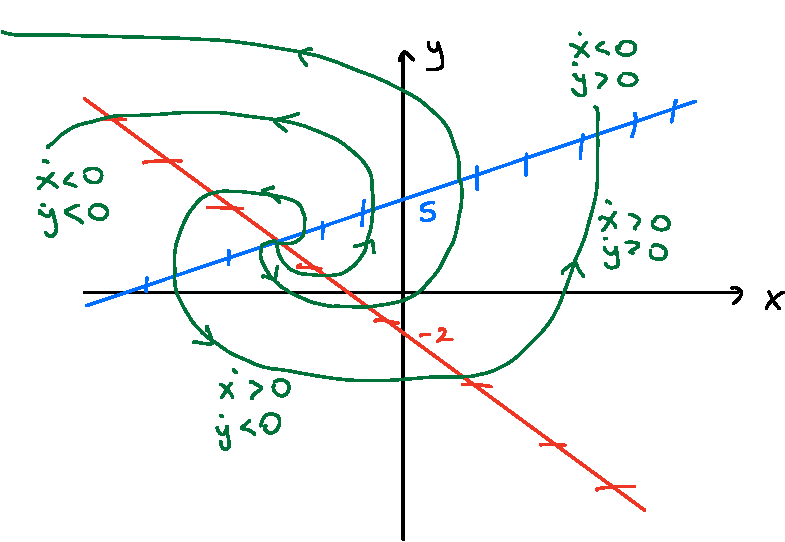
\includegraphics[width=13cm]{images/nullclines-ps1.pdf}
      \end{center}
    }

    %\section{SIR with temporary immunity}
    %So far, we have assumed that immunity is permanent (how has this been encoded into our model?) What if immunity is only temporary? This is a concern about Covid-19.
    %\begin{enumerate}[label=(\alph*)]
    %  \item Introduce a new term to our equations which represents the `movement' of the population from the immune section, $R$, to the susceptible section, $S$.
    %  \item Show that there are two equilibria of this new model, with one of them given by
    %  \begin{equation}
    %    S = \frac{\gamma}{\beta}, \quad I = \frac{N-\frac{\gamma}{\beta}}{1 + \frac{\gamma}{\delta}}, \quad R = \frac{N-\frac{\gamma}{\beta}}{1 + \frac{\delta}{\gamma}},
    %  \end{equation}
    %  where $\delta$ is the factor on your $R$ terms in the governing equations. Is this different to our original SIR model, and if so, how?
    %  \item By using the equation for $N$ to eliminate $R$ from your expression for $\fd{S}{t}$, write down two equations governing this system.
    %  \item By writing down the Jacobian of this reduced system where appropriate, perform a linear stability analysis on the equilibria you have found, and state under what conditions each equilibria is asymptotically stable/unstable/degenerate. (Hint: you may find the rules about determinants and traces useful.)
    %  \item How might you explain this to the general public? (Assuming you are able to crop your slides to the correct aspect ratio.)
    %\end{enumerate}

    %\section{SIR with natural birth and death}
    %We now return to our original SIR model, but add in natural birth and death. We haven't added this in so far (why might that be OK?) but don't forget that these terms also represent immigration and emigration: a rush of Londoners travelling to their second homes in Cornwall, for example.
    %\begin{enumerate}[label=(\alph*)]
    %  \item Add new terms to the original SIR system to model this new situation. (Be careful: natural death affects everybody!)
    %  \item In order to have a constant population ($\fd{N}{t} = 0$), what must we assume about the birth and death rates?
    %  \item Find the equilibria of this new model, and compare these to the models we have found so far.
    %  \item By considering the sub-system consisting of the equations for $\fd{S}{t}$ and $\fd{I}{t}$, once again write down the Jacobian and perform a linear stability analysis on these equilibria. What is $R_0$ in this new model?
    %\end{enumerate}
    %
    %\section{SEIR models}
    %For many diseases, there is an incubation period where the individual is infect\emph{ed} but not yet infect\emph{ious}.
    %\begin{enumerate}[label=(\alph*)]
    %  \item Keeping the natural birth and death terms from your previous model, add in a new class $E$ for the `exposed' population, so that the population goes through the process in the order
    %  \[ S \to E \to I \to R.\]
    %  \item Show that in this model, the basic reproduction number $R_0$ is given by
    %  \begin{equation}
    %    R_0 = \frac{\alpha\beta}{(\mu+\alpha)(\mu+\gamma)},
    %  \end{equation}
    %  where $\mu$ is the birth/death rate, $\alpha$ is your $E$ rate, $\beta$ is your $SI$ rate, and $\gamma$ is your $I$ rate.
    %\end{enumerate}
    %%Next time... vaccines.

\end{enumerate}
\end{document}
